\documentclass[12pt,a4paper]{article}
\usepackage[utf8]{inputenc}
\usepackage[norsk]{babel}  % Norwegian language support
\usepackage[margin=1in]{geometry}
\usepackage{graphicx}
\usepackage{float}
\usepackage{hyperref}
\usepackage{listings}
\usepackage{xcolor}
\usepackage{fancyhdr}
\usepackage{pdflscape}  % For landscape pages
\usepackage{afterpage}  % For better page breaks
\usepackage{adjustbox}  % For better image scaling control

% Fix headheight warning
\setlength{\headheight}{14.49998pt}

% Code listing settings
\lstset{
    basicstyle=\ttfamily\small,
    breaklines=true,
    frame=single,
    numbers=left,
    numberstyle=\tiny\color{gray},
    backgroundcolor=\color{gray!10},
    keywordstyle=\color{blue}\bfseries,
    commentstyle=\color{green!60!black},
    stringstyle=\color{red}
}

% Hyperlink settings
\hypersetup{
    colorlinks=true,
    linkcolor=blue,
    urlcolor=cyan,
}

% Header/Footer
\pagestyle{fancy}
\fancyhf{}
\rhead{Assignment 3 - User Authentication}
\lhead{Gruppe 2}
\rfoot{\thepage}

\begin{document}

% Title Page
\begin{titlepage}
    \centering
    \vspace*{1cm}

    \vspace{1.5cm}

    {\Huge\bfseries Assignment 3 - User Authentication\par}

    \vspace{1cm}

    {\Large Gruppe 2\par}

    \vspace{0.5cm}

    {\large av\par}

    \vspace{0.5cm}

    {\large Bjarte Wik, Brage Evjen, Matias Garatun, Tor Martin Tobiassen Kohle\par}

    \vspace{1cm}

    {\large i\par}

    \vspace{0.5cm}

    {\large IKT222-G 25H\par}
    {\large Software Sikkerhet\par}

    \vspace{1.5cm}

    {\large Fakultet for teknologi og realfag\par}
    {\large Universitetet i Agder\par}

    \vfill

    {\large Grimstad, oktober 2025\par}

\end{titlepage}

\tableofcontents
\newpage

\section{Overview}

We extended our recipe sharing application from Assignment 2 with a comprehensive authentication system. The system implements OAuth2 Authorization Code Flow with PKCE, conventional username/password authentication, Two-Factor Authentication (TOTP), brute force protection, and a secure database backend.

\subsection{Application Architecture}

The application is built with Flask and SQLite, organized into three route blueprints (auth, oauth, twofa), five singleton services, and a database with 9 tables. Figure \ref{fig:architecture} shows the complete architecture with file:line references from the source code.

\begin{figure}[H]
    \centering
    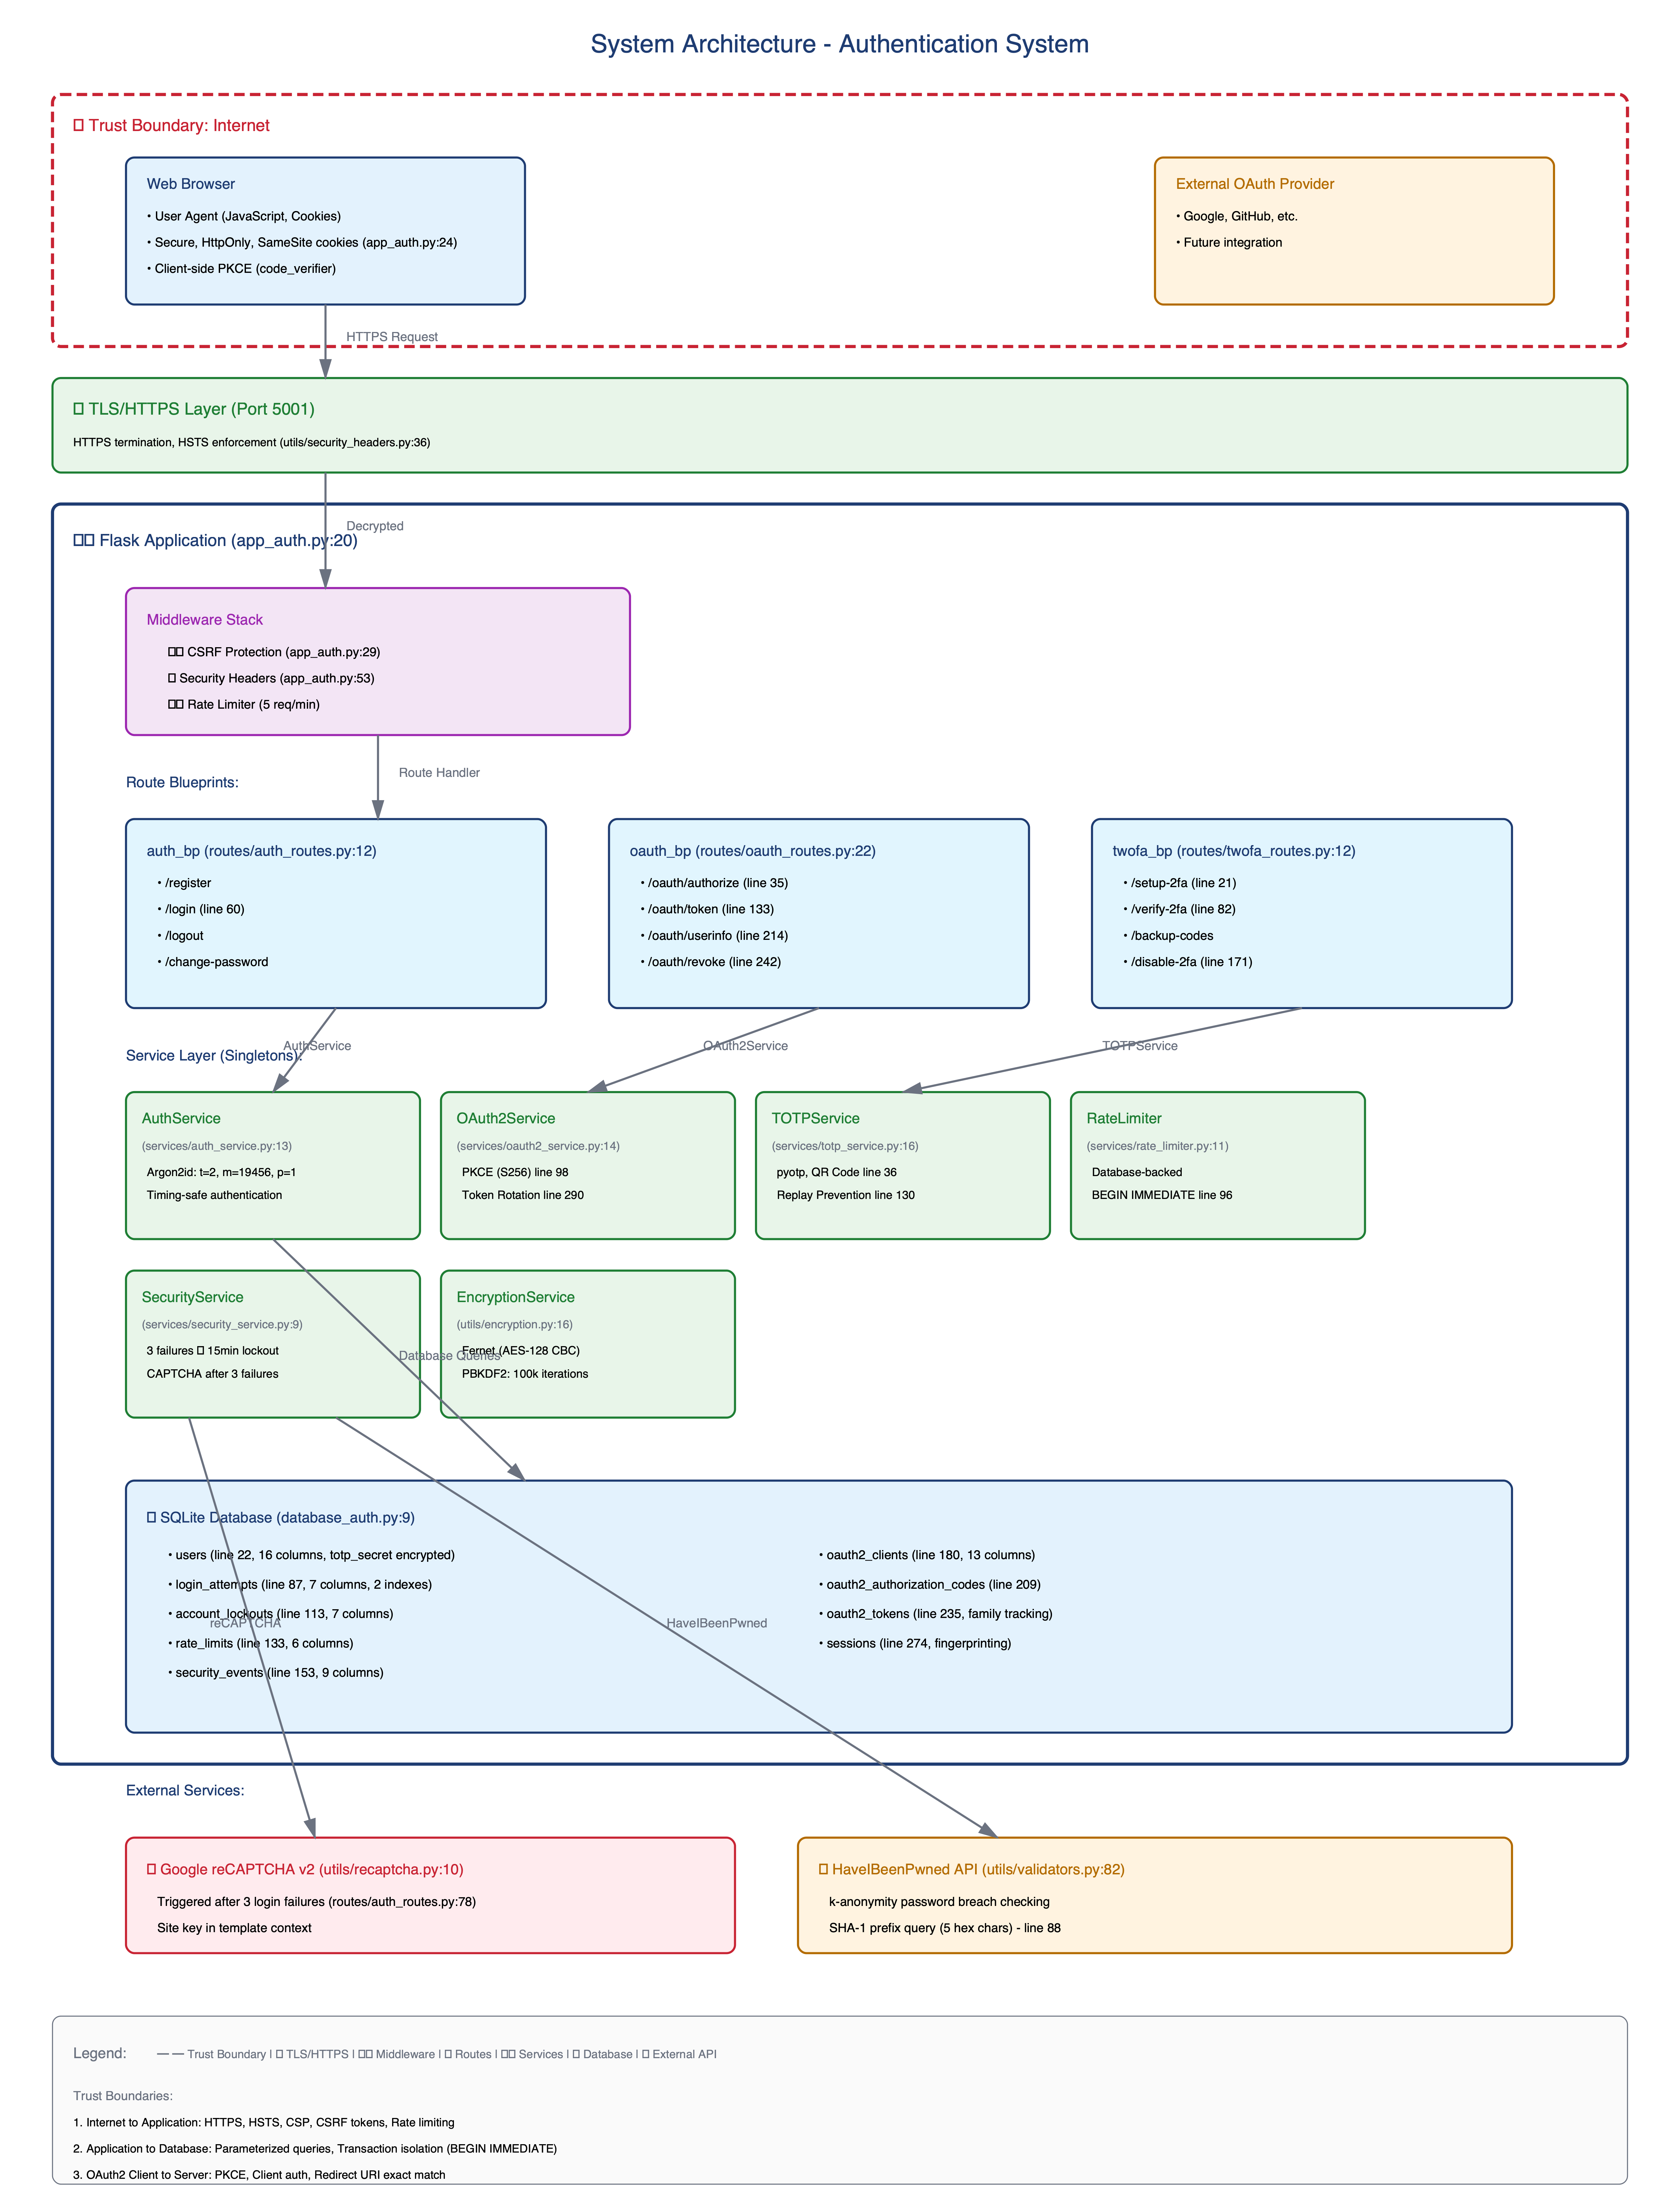
\includegraphics[width=\textwidth,height=0.85\textheight,keepaspectratio]{diagrams/1_system_architecture.png}
    \caption{System Architecture with middleware stack, route blueprints, services, and external integrations}
    \label{fig:architecture}
\end{figure}

The architecture includes middleware for CSRF protection, security headers, and rate limiting. External integrations include Google reCAPTCHA for bot prevention and Have I Been Pwned API for password breach detection.

\section{Task 1: Database Integration}

\subsection{Database Schema}

We designed a SQLite database with 9 tables, 15 indexes, and 8 foreign key relationships with CASCADE delete behavior. The schema supports all required authentication features while maintaining data integrity and performance.

\begin{figure}[H]
    \centering
    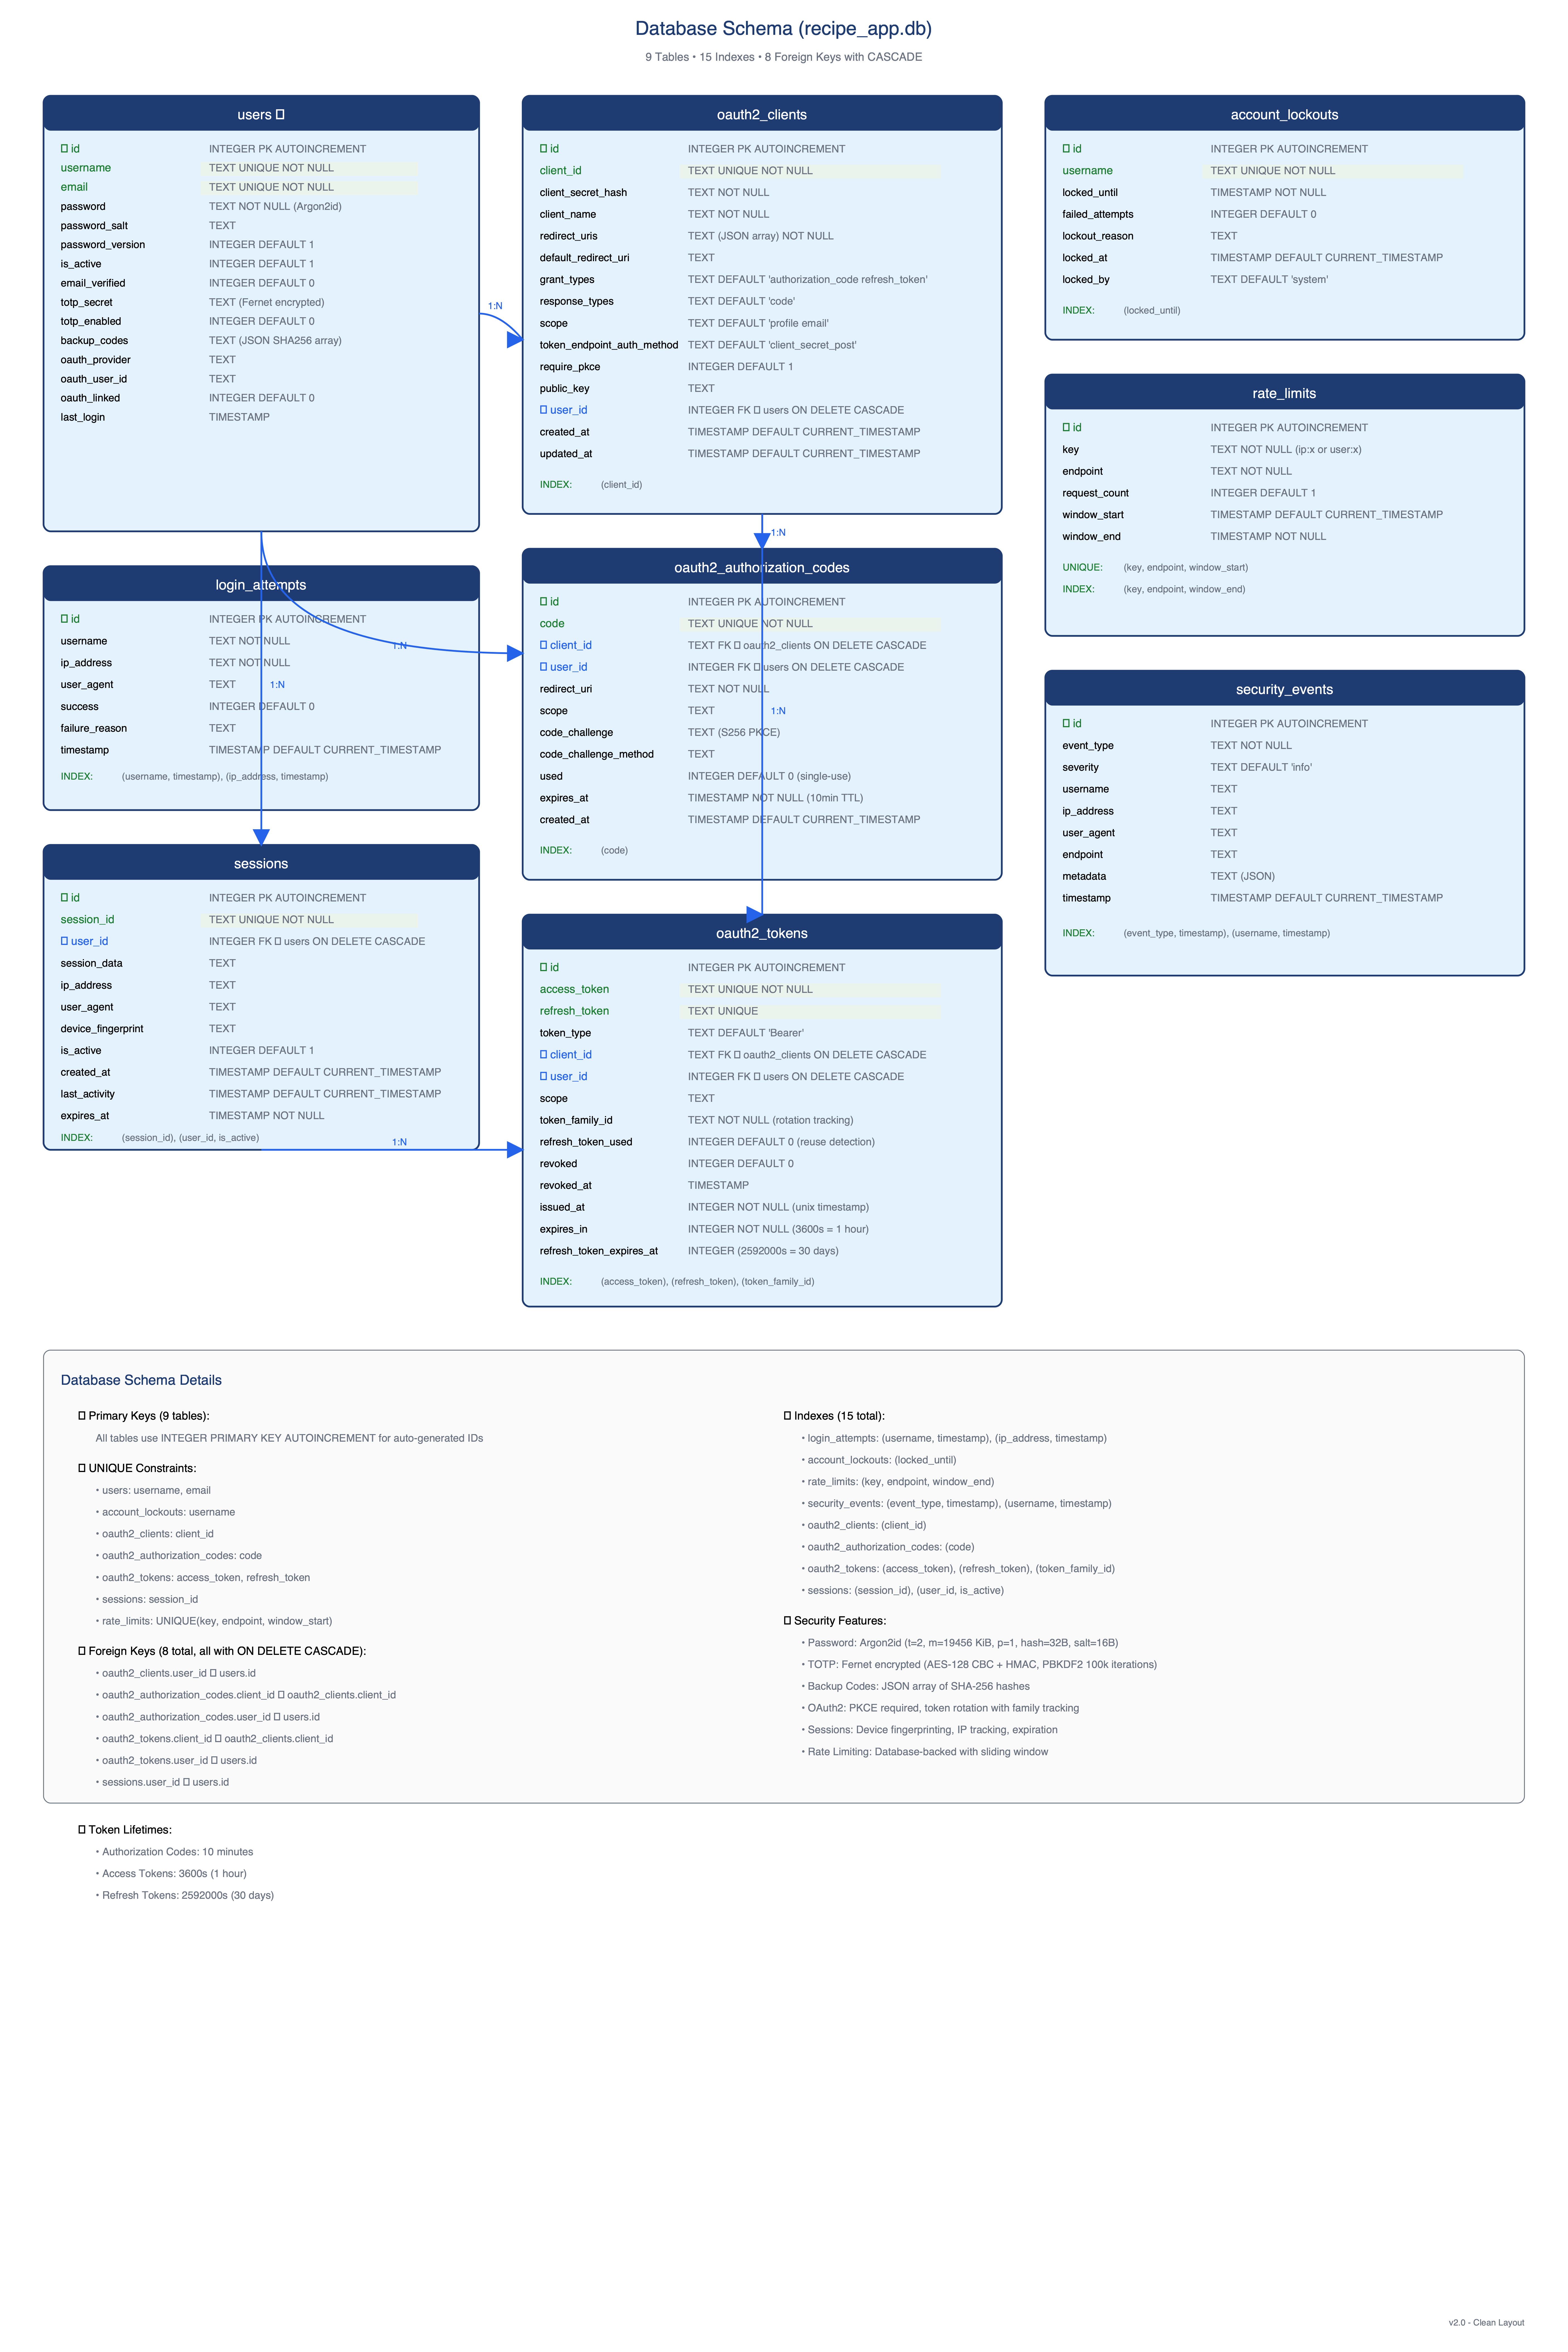
\includegraphics[width=\textwidth,height=0.9\textheight,keepaspectratio]{diagrams/4_database_er.png}
    \caption{Entity-Relationship Diagram showing all 9 tables with foreign key constraints}
    \label{fig:database}
\end{figure}

The database includes core authentication tables (users, login\_attempts, account\_lockouts, rate\_limits, security\_events), OAuth2 tables (oauth2\_clients, oauth2\_authorization\_codes, oauth2\_tokens), and session management. The users table has 16 columns including encrypted TOTP secrets and OAuth linking fields.

\subsection{Security Challenges and Mitigations}

\textbf{Challenge 1: SQL Injection}

Direct string concatenation allows attackers to inject malicious SQL. We prevent this using parameterized queries exclusively:

\begin{lstlisting}[language=Python]
# SECURE: Parameterized query
cursor.execute('SELECT * FROM users WHERE username = ?', (username,))
\end{lstlisting}

\textbf{Challenge 2: Race Conditions}

Multiple concurrent requests could create TOCTOU vulnerabilities. We use \texttt{BEGIN IMMEDIATE} transactions to acquire write locks immediately at 4 critical locations: authorization code validation, refresh token rotation, account lockout application, and rate limit recording.

\textbf{Challenge 3: Sensitive Data Exposure}

Sensitive data is protected with multiple encryption methods:
\begin{itemize}
    \item Passwords: Argon2id (memory-hard, GPU-resistant)
    \item TOTP secrets: Fernet encryption (AES-128 CBC + HMAC)
    \item Backup codes: SHA-256 hashing
    \item OAuth secrets: bcrypt hashing
\end{itemize}

\section{Task 2: Basic User Authentication}

\subsection{Password Hashing with Argon2id}

We use Argon2id with OWASP-recommended parameters \cite{owasp_password}. Argon2id won the Password Hashing Competition in 2015 \cite{biryukov2016} and is memory-hard, preventing GPU/ASIC acceleration.

\begin{lstlisting}[language=Python]
self.hasher = PasswordHasher(
    time_cost=2,         # 2 iterations
    memory_cost=19456,   # 19 MiB
    parallelism=1,
    hash_len=32,
    salt_len=16          # Auto-generated
)
\end{lstlisting}

\subsection{HIBP Breach Detection}

We integrate with Have I Been Pwned using the k-anonymity model. Only the first 5 characters of the SHA-1 hash are sent to HIBP, protecting user privacy:

\begin{lstlisting}[language=Python]
sha1 = hashlib.sha1(password.encode()).hexdigest().upper()
prefix, suffix = sha1[:5], sha1[5:]

response = requests.get(
    f'https://api.pwnedpasswords.com/range/{prefix}'
)

# Check if full hash appears in breached passwords
for line in response.text.splitlines():
    hash_suffix, count = line.split(':')
    if hash_suffix == suffix:
        return True, int(count)  # Breached!
\end{lstlisting}

\begin{figure}[H]
    \centering
    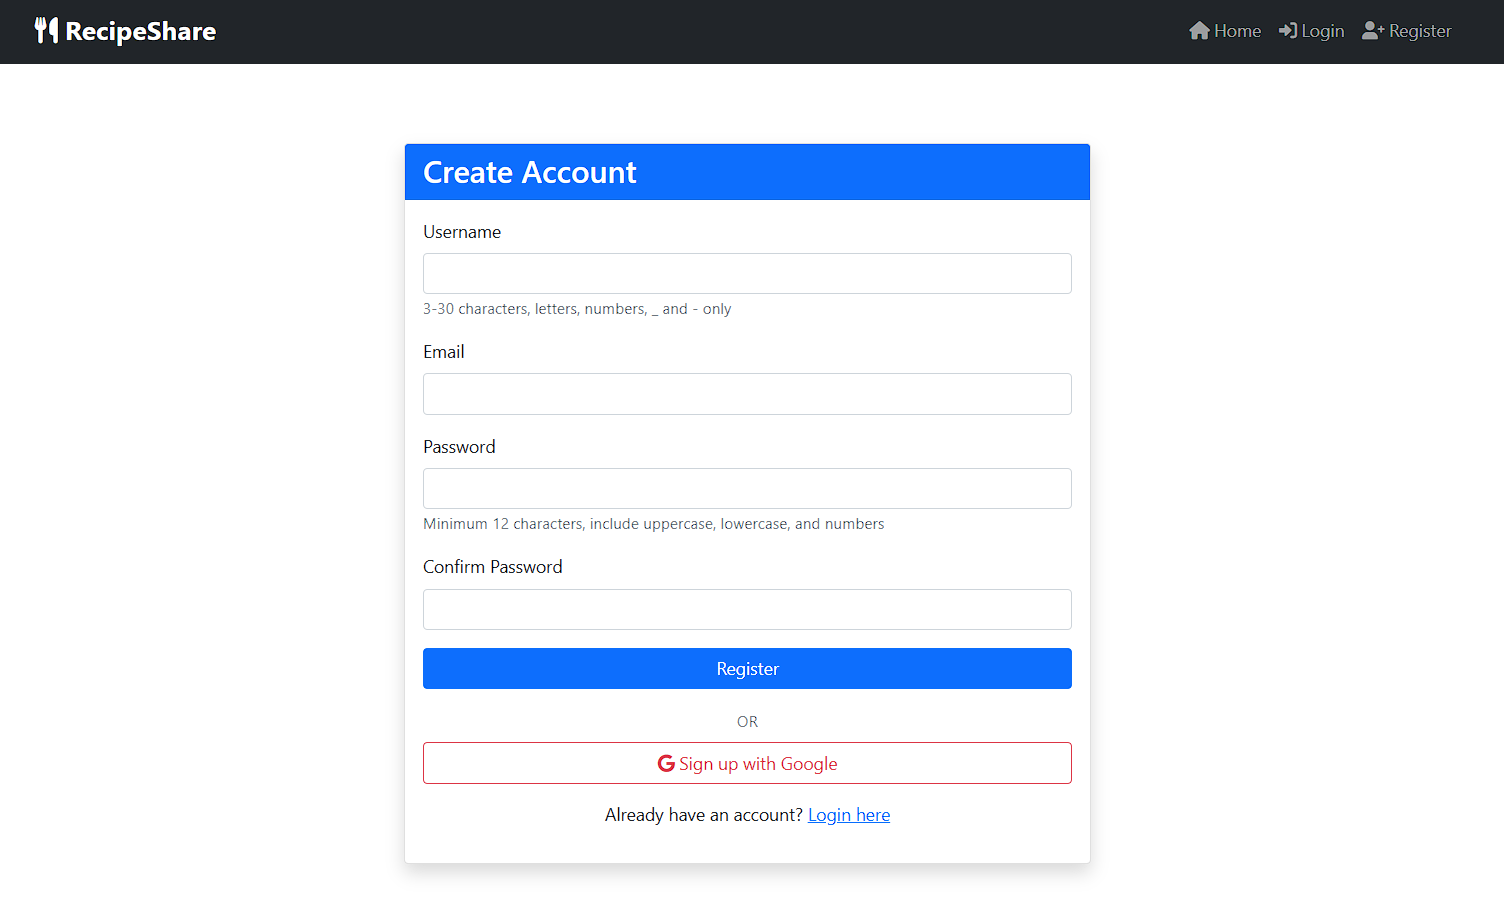
\includegraphics[width=0.85\textwidth]{SCREENSHOTs/Register.png}
    \caption{Registration form with HIBP password breach detection showing error message when user attempts to use a compromised password}
    \label{fig:hibp}
\end{figure}

\subsection{Security Challenges and Mitigations}

\textbf{Challenge 1: Timing Attacks}

Attackers can determine if a username exists by measuring response times.

\textbf{Mitigation}: We perform dummy hash operations when usernames don't exist, ensuring constant-time responses regardless of username validity.

\textbf{Challenge 2: Session Fixation}

Attackers could set a victim's session ID before authentication.

\textbf{Mitigation}: Session regeneration at two critical points: after password authentication and after 2FA verification.

\section{Task 3: Protection Against Brute Force Attacks}

\subsection{Three-Layer Defense}

We implement rate limiting, account lockout, and CAPTCHA challenges as complementary defense layers. Figure \ref{fig:brute_force} shows the complete protection flow.

\begin{figure}[H]
    \centering
    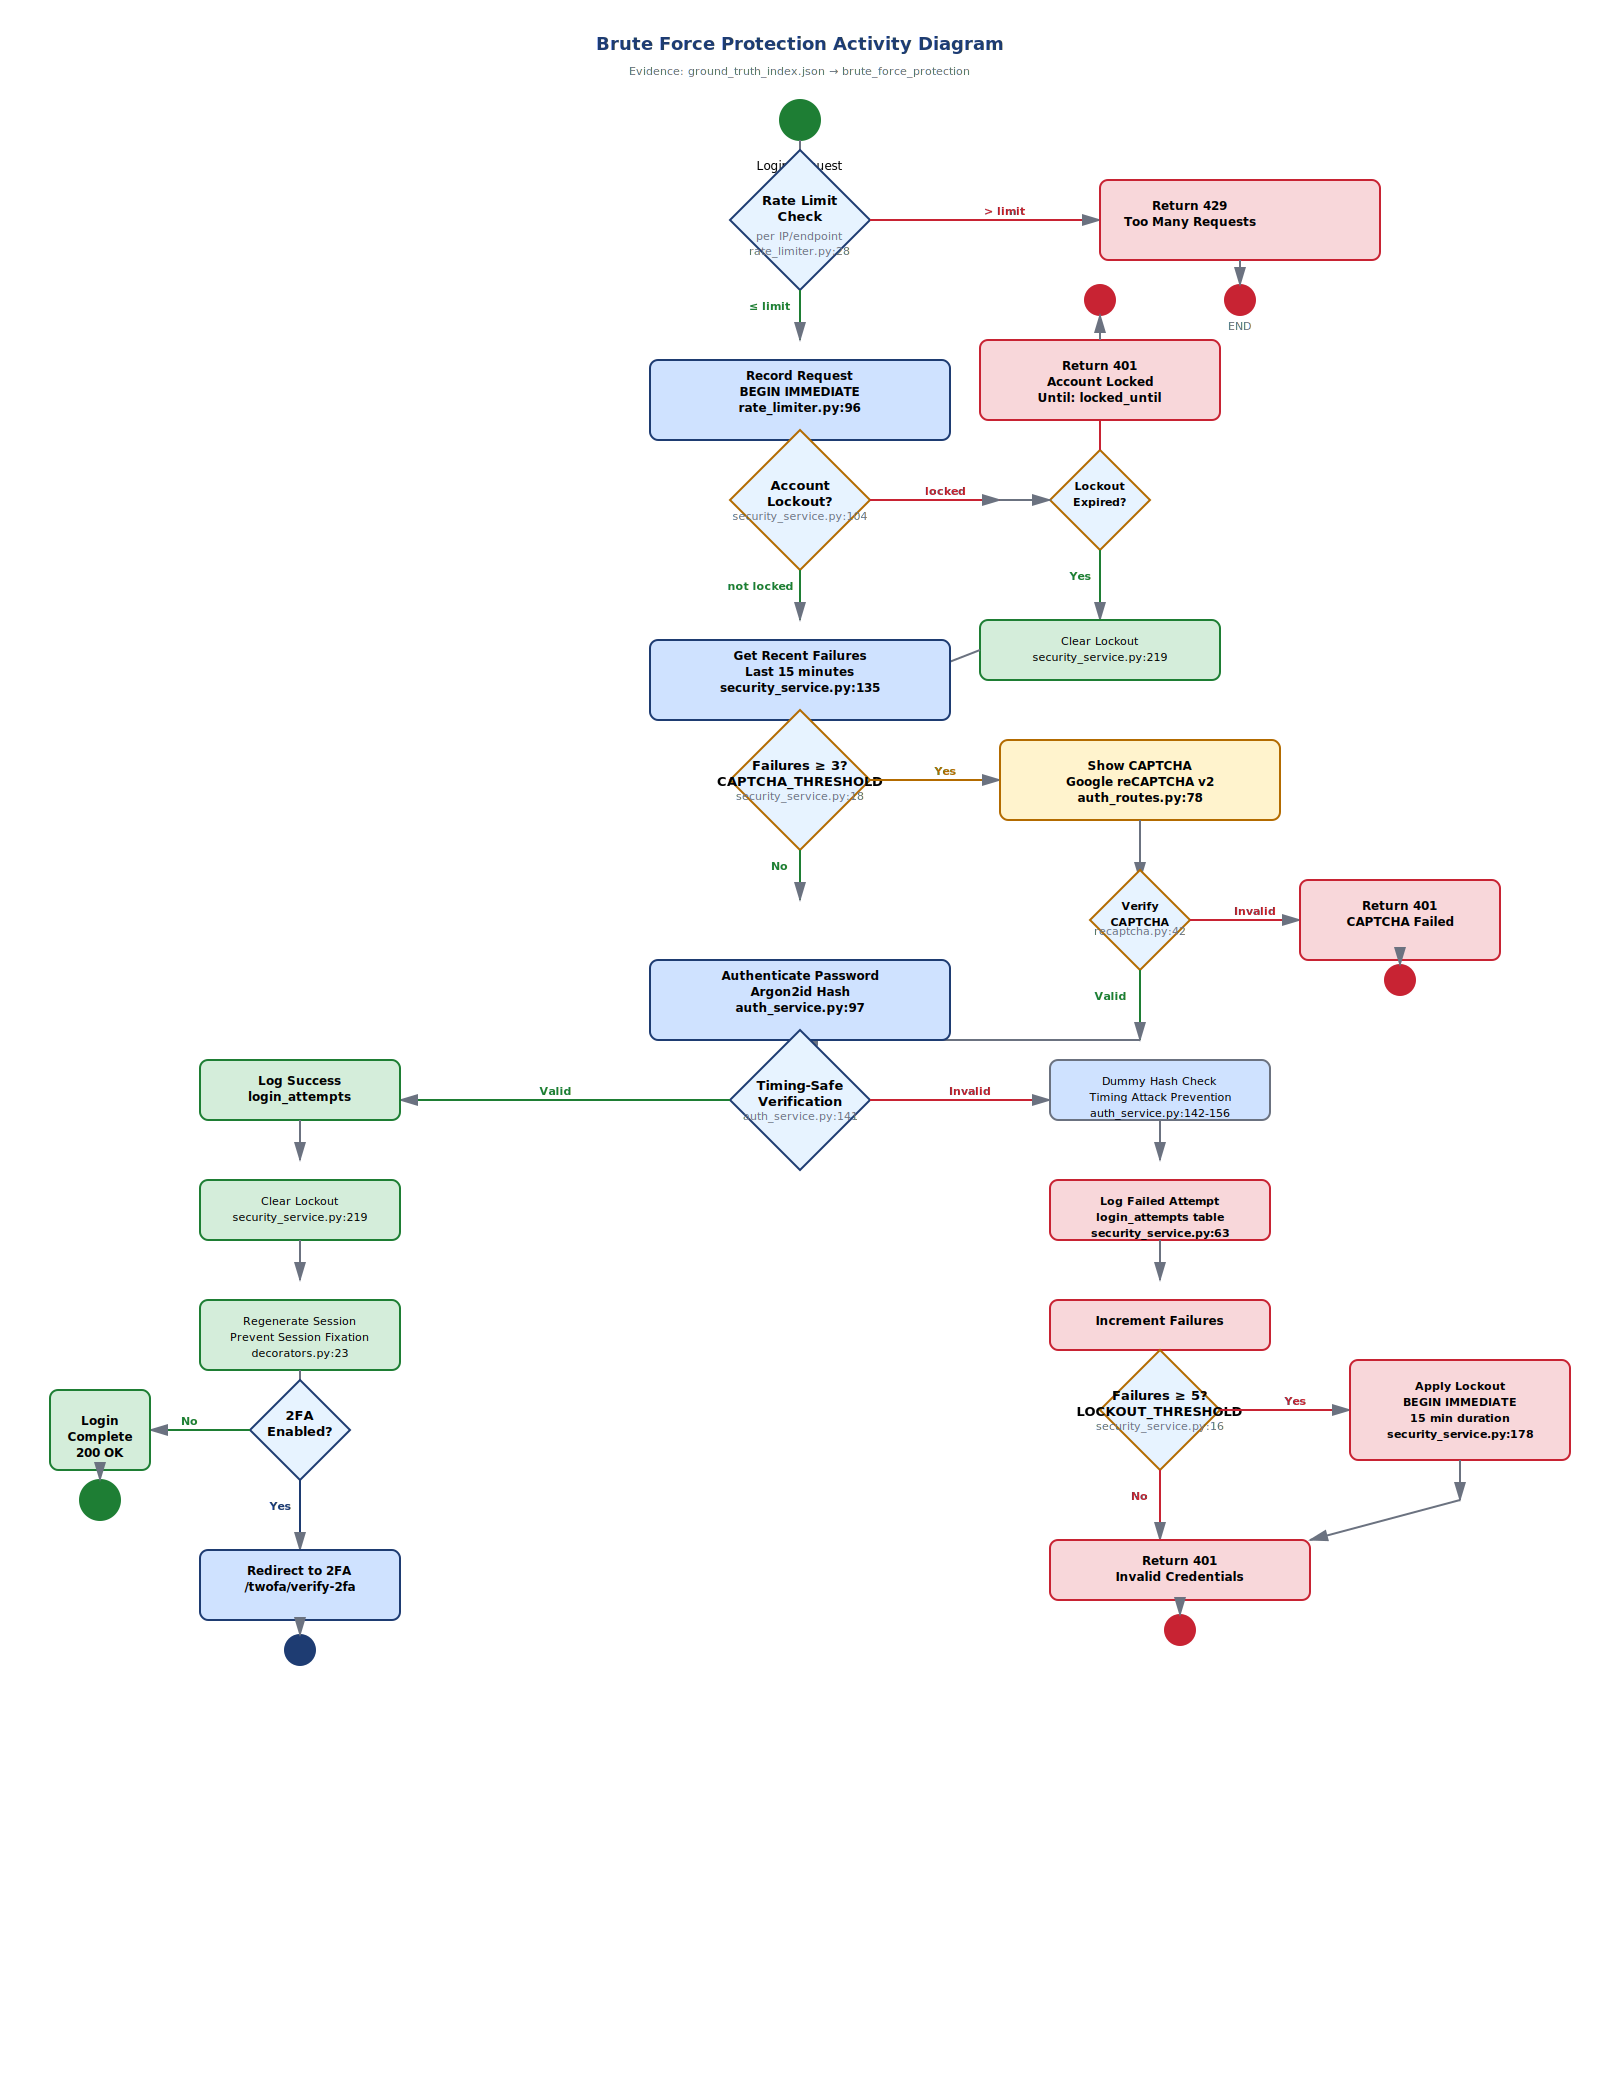
\includegraphics[width=\textwidth,height=0.85\textheight,keepaspectratio]{diagrams/6_brute_force_activity.png}
    \caption{Brute Force Protection Activity Diagram showing rate limiting, lockout checks, and CAPTCHA}
    \label{fig:brute_force}
\end{figure}

\textbf{Layer 1: Rate Limiting} - Database-backed, 5 requests per minute per user, returns HTTP 429 when exceeded.

\textbf{Layer 2: Account Lockout} - After 5 failed attempts within 15 minutes, accounts are locked for 15 minutes. Figure \ref{fig:lockout_state} shows the state transitions.

\begin{figure}[H]
    \centering
    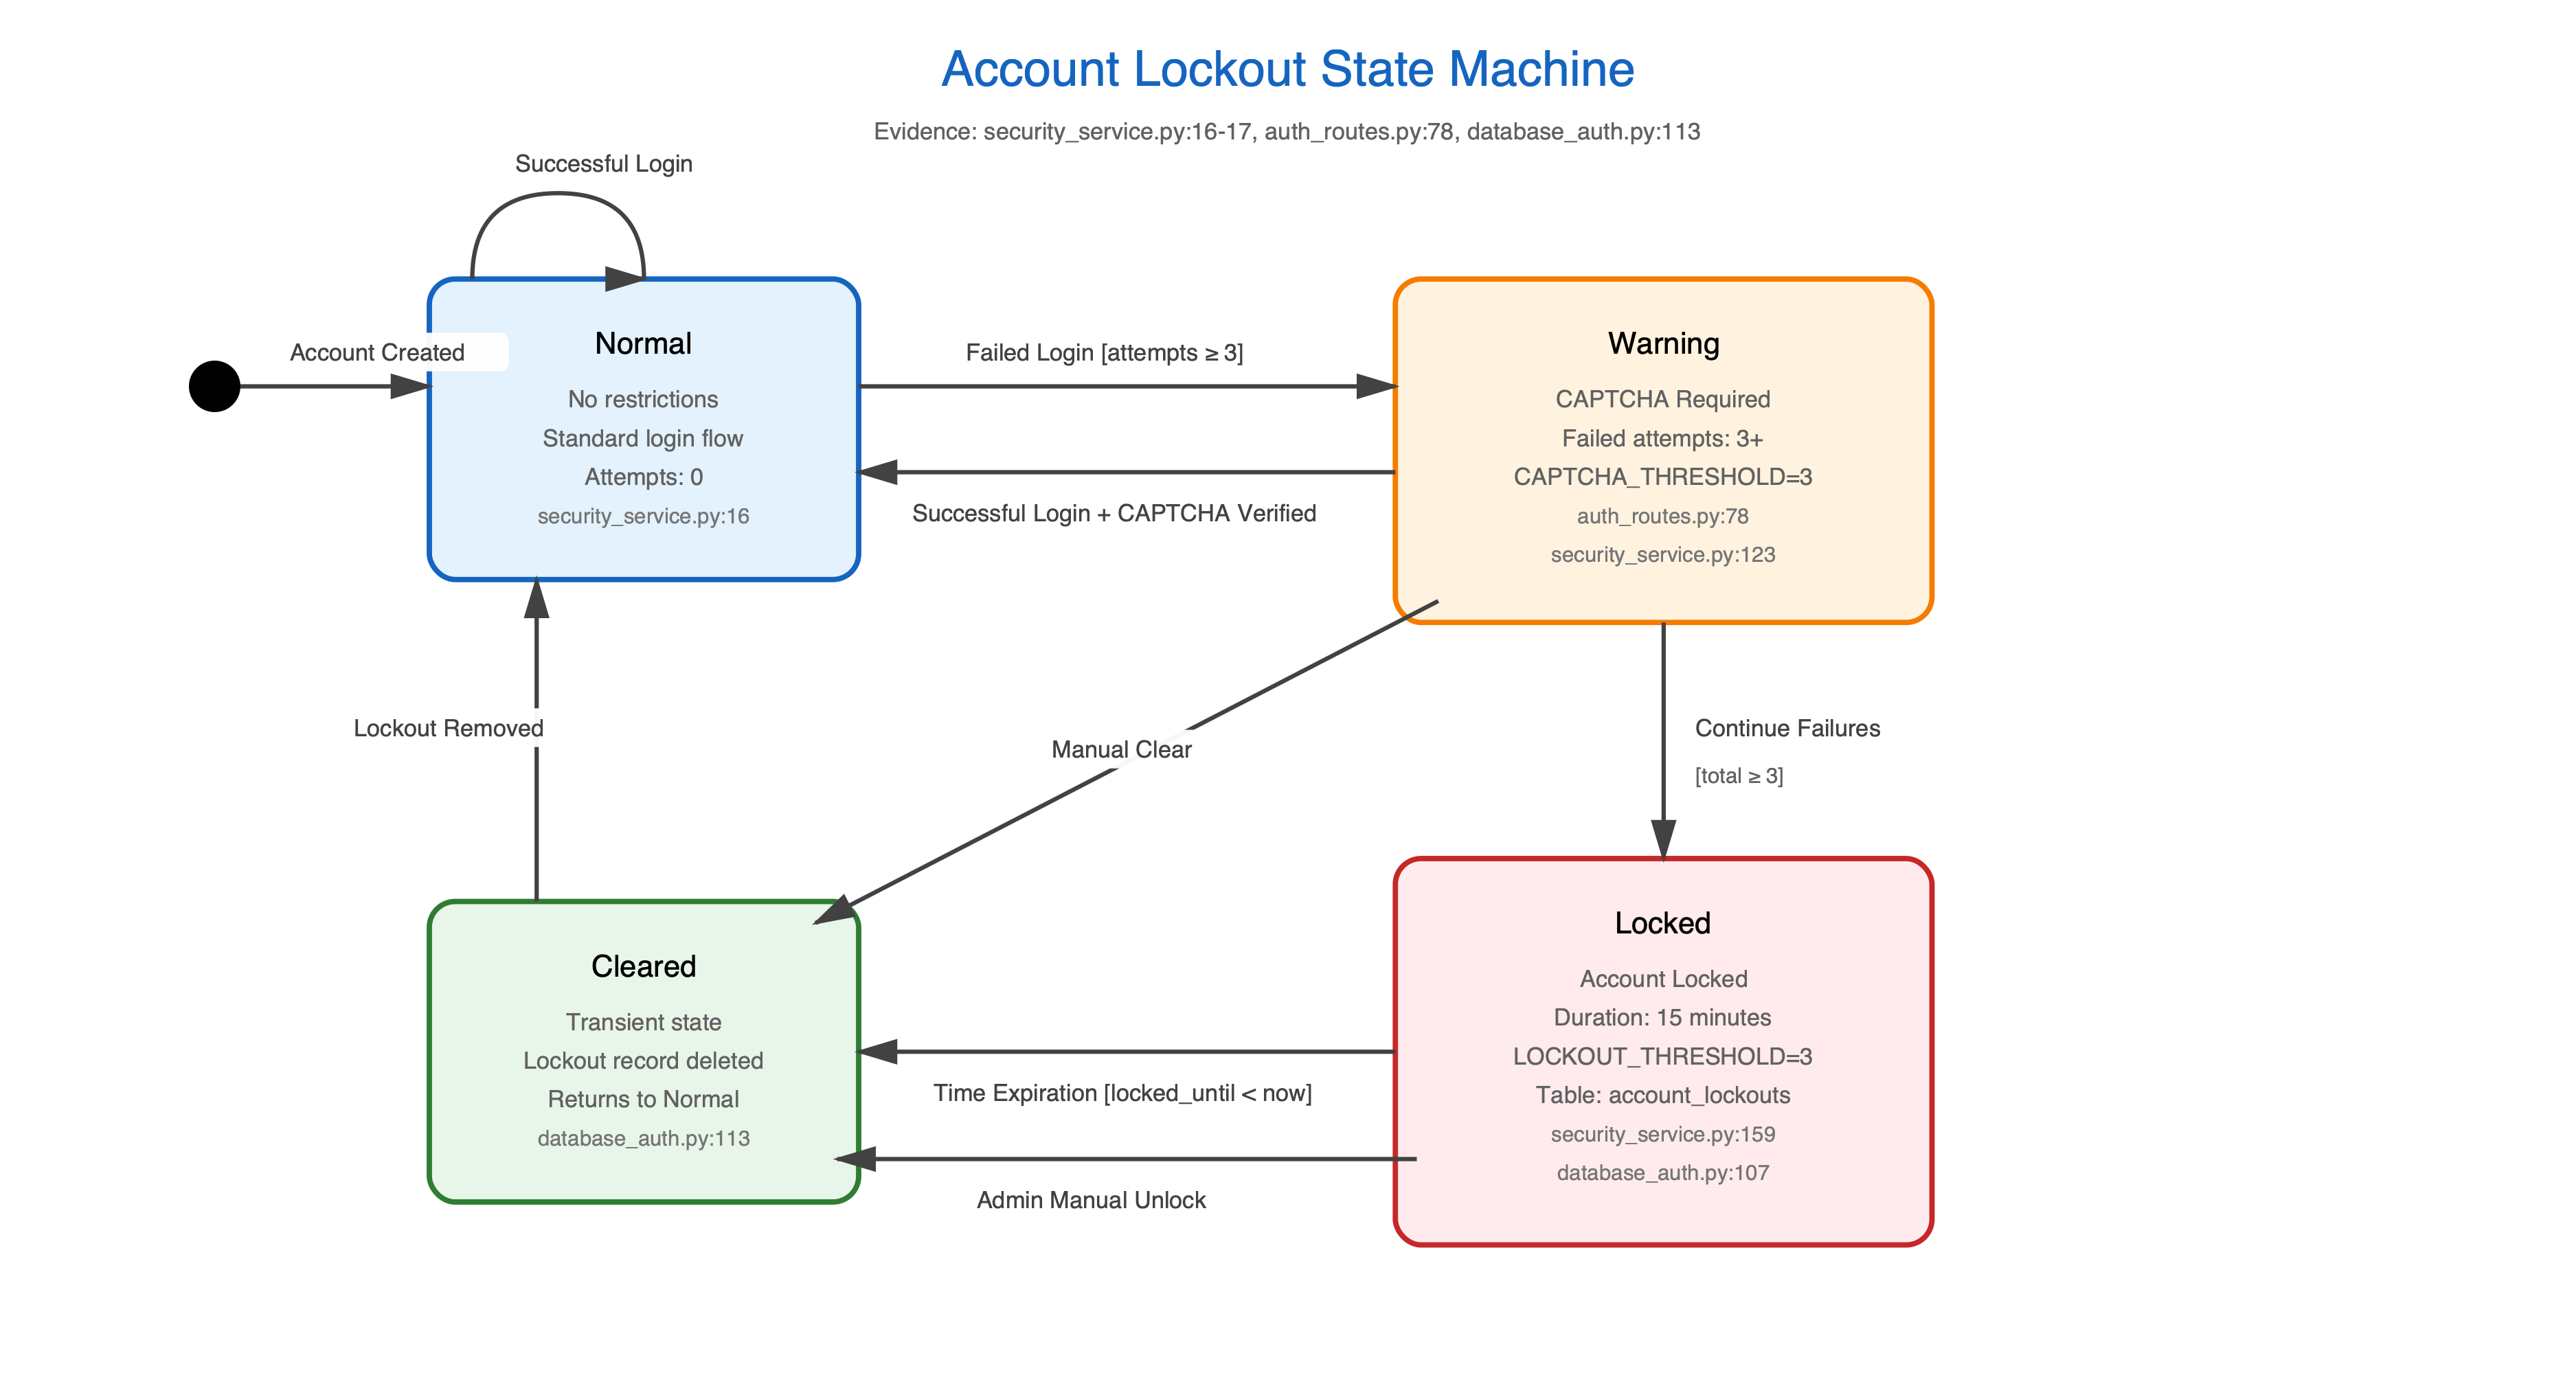
\includegraphics[width=\textwidth,keepaspectratio]{diagrams/13_account_lockout_state_machine.png}
    \caption{Account Lockout State Machine}
    \label{fig:lockout_state}
\end{figure}

\textbf{Layer 3: CAPTCHA} - Google reCAPTCHA v2 required after 3 failures, prevents automated attacks.

\begin{figure}[H]
    \centering
    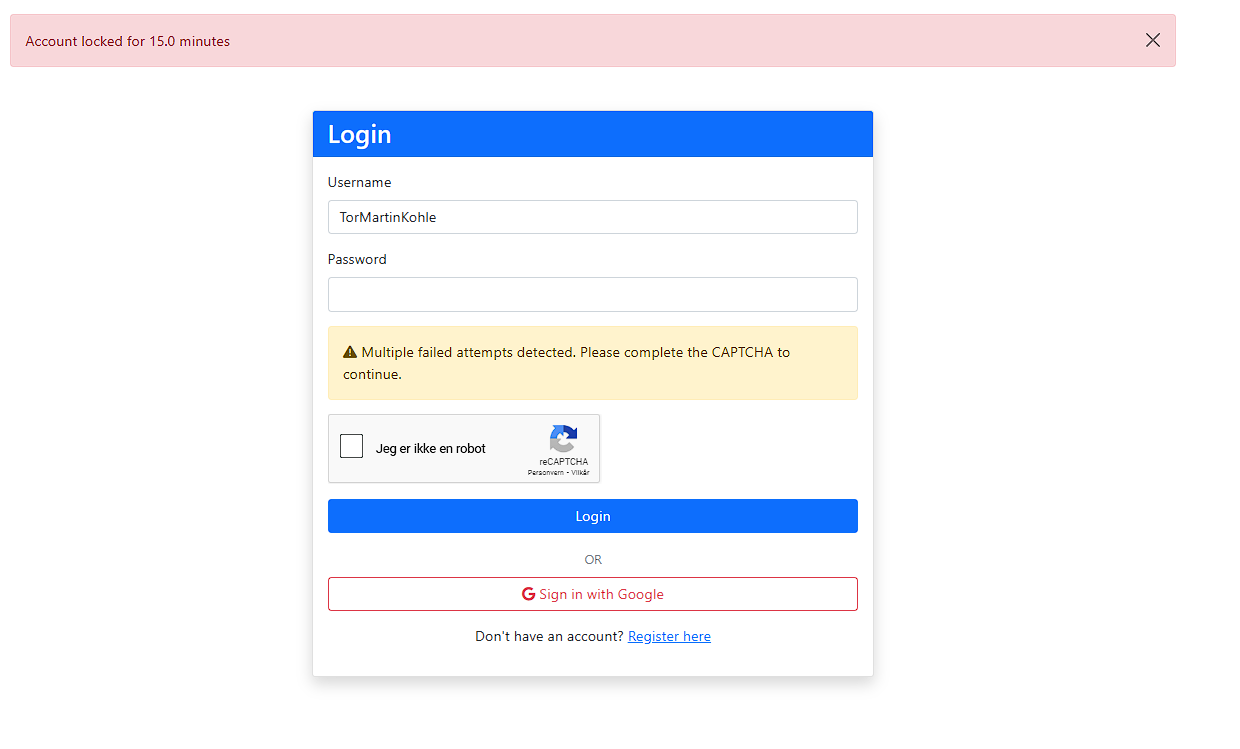
\includegraphics[width=0.85\textwidth]{SCREENSHOTs/account locked.png}
    \caption{Account lockout message after 5 failed login attempts}
    \label{fig:lockout_screen}
\end{figure}

\begin{figure}[H]
    \centering
    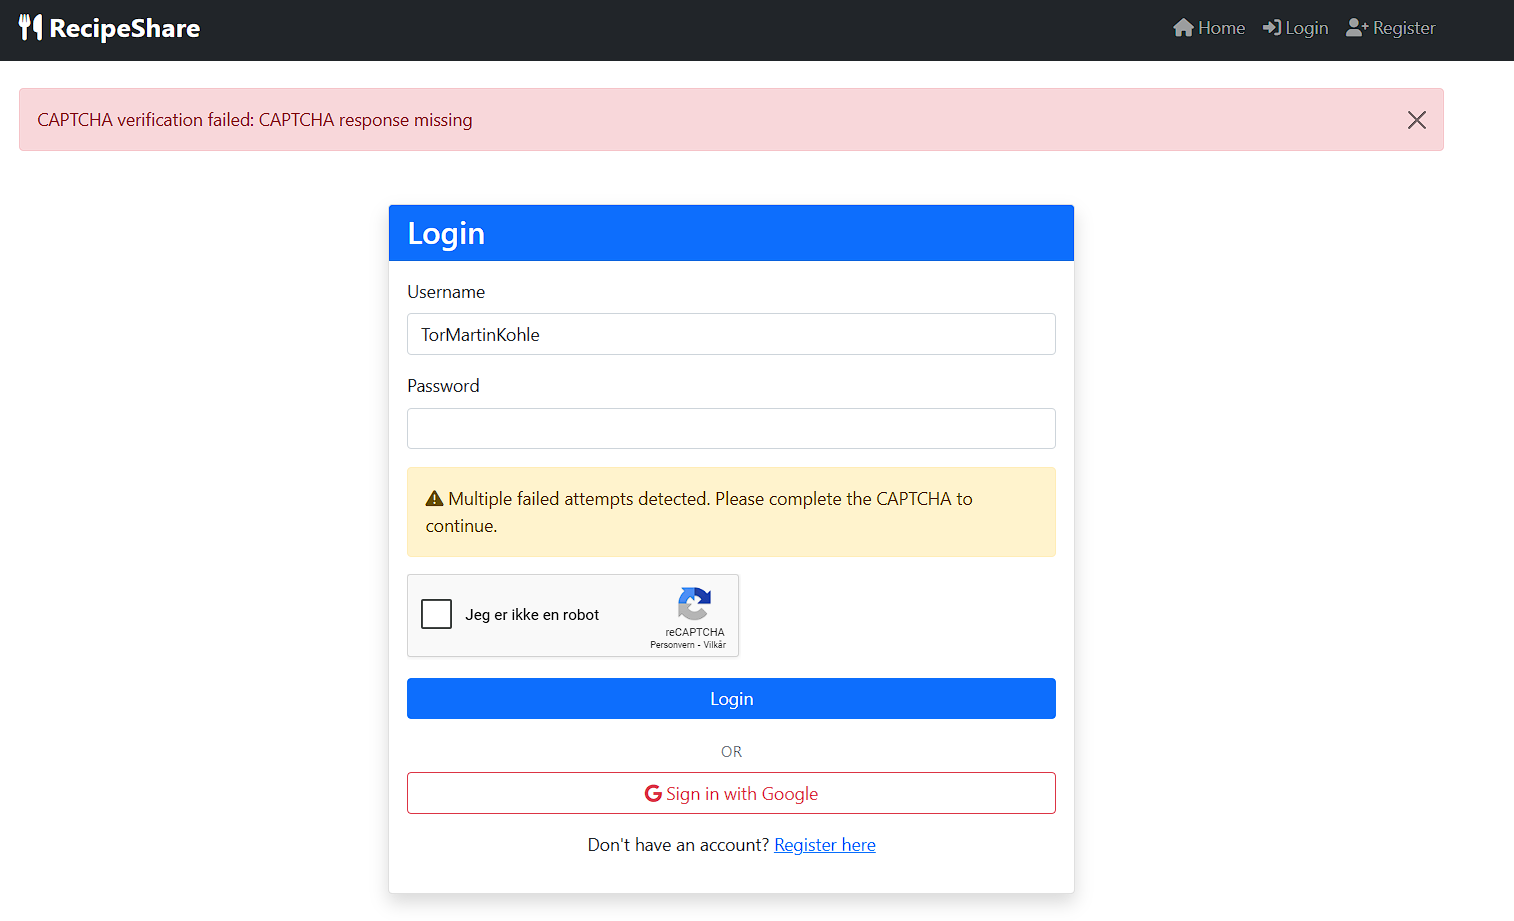
\includegraphics[width=0.85\textwidth]{SCREENSHOTs/reCaptcha.png}
    \caption{Google reCAPTCHA v2 checkbox challenge after 3 failed attempts}
    \label{fig:captcha}
\end{figure}

\subsection{Security Challenges and Mitigations}

\textbf{Challenge 1: Distributed Brute Force}

Attackers using multiple IPs could bypass per-IP rate limiting.

\textbf{Mitigation}: Per-user rate limiting based on username in form data prevents distributed attacks on a single account.

\textbf{Challenge 2: Denial of Service}

Attackers could intentionally lock out legitimate users.

\textbf{Mitigation}: Short 15-minute lockout duration minimizes DoS impact while preventing brute force. Security events are logged for abuse detection.

\section{Task 4: Two-Factor Authentication}

\subsection{TOTP Implementation}

We implement Time-based One-Time Passwords according to RFC 6238 \cite{mraihi2011} using the pyotp library. Users scan a QR code with Google Authenticator or similar apps. The complete 2FA flow is shown in Figure \ref{fig:2fa_flow}.

\begin{figure}[H]
    \centering
    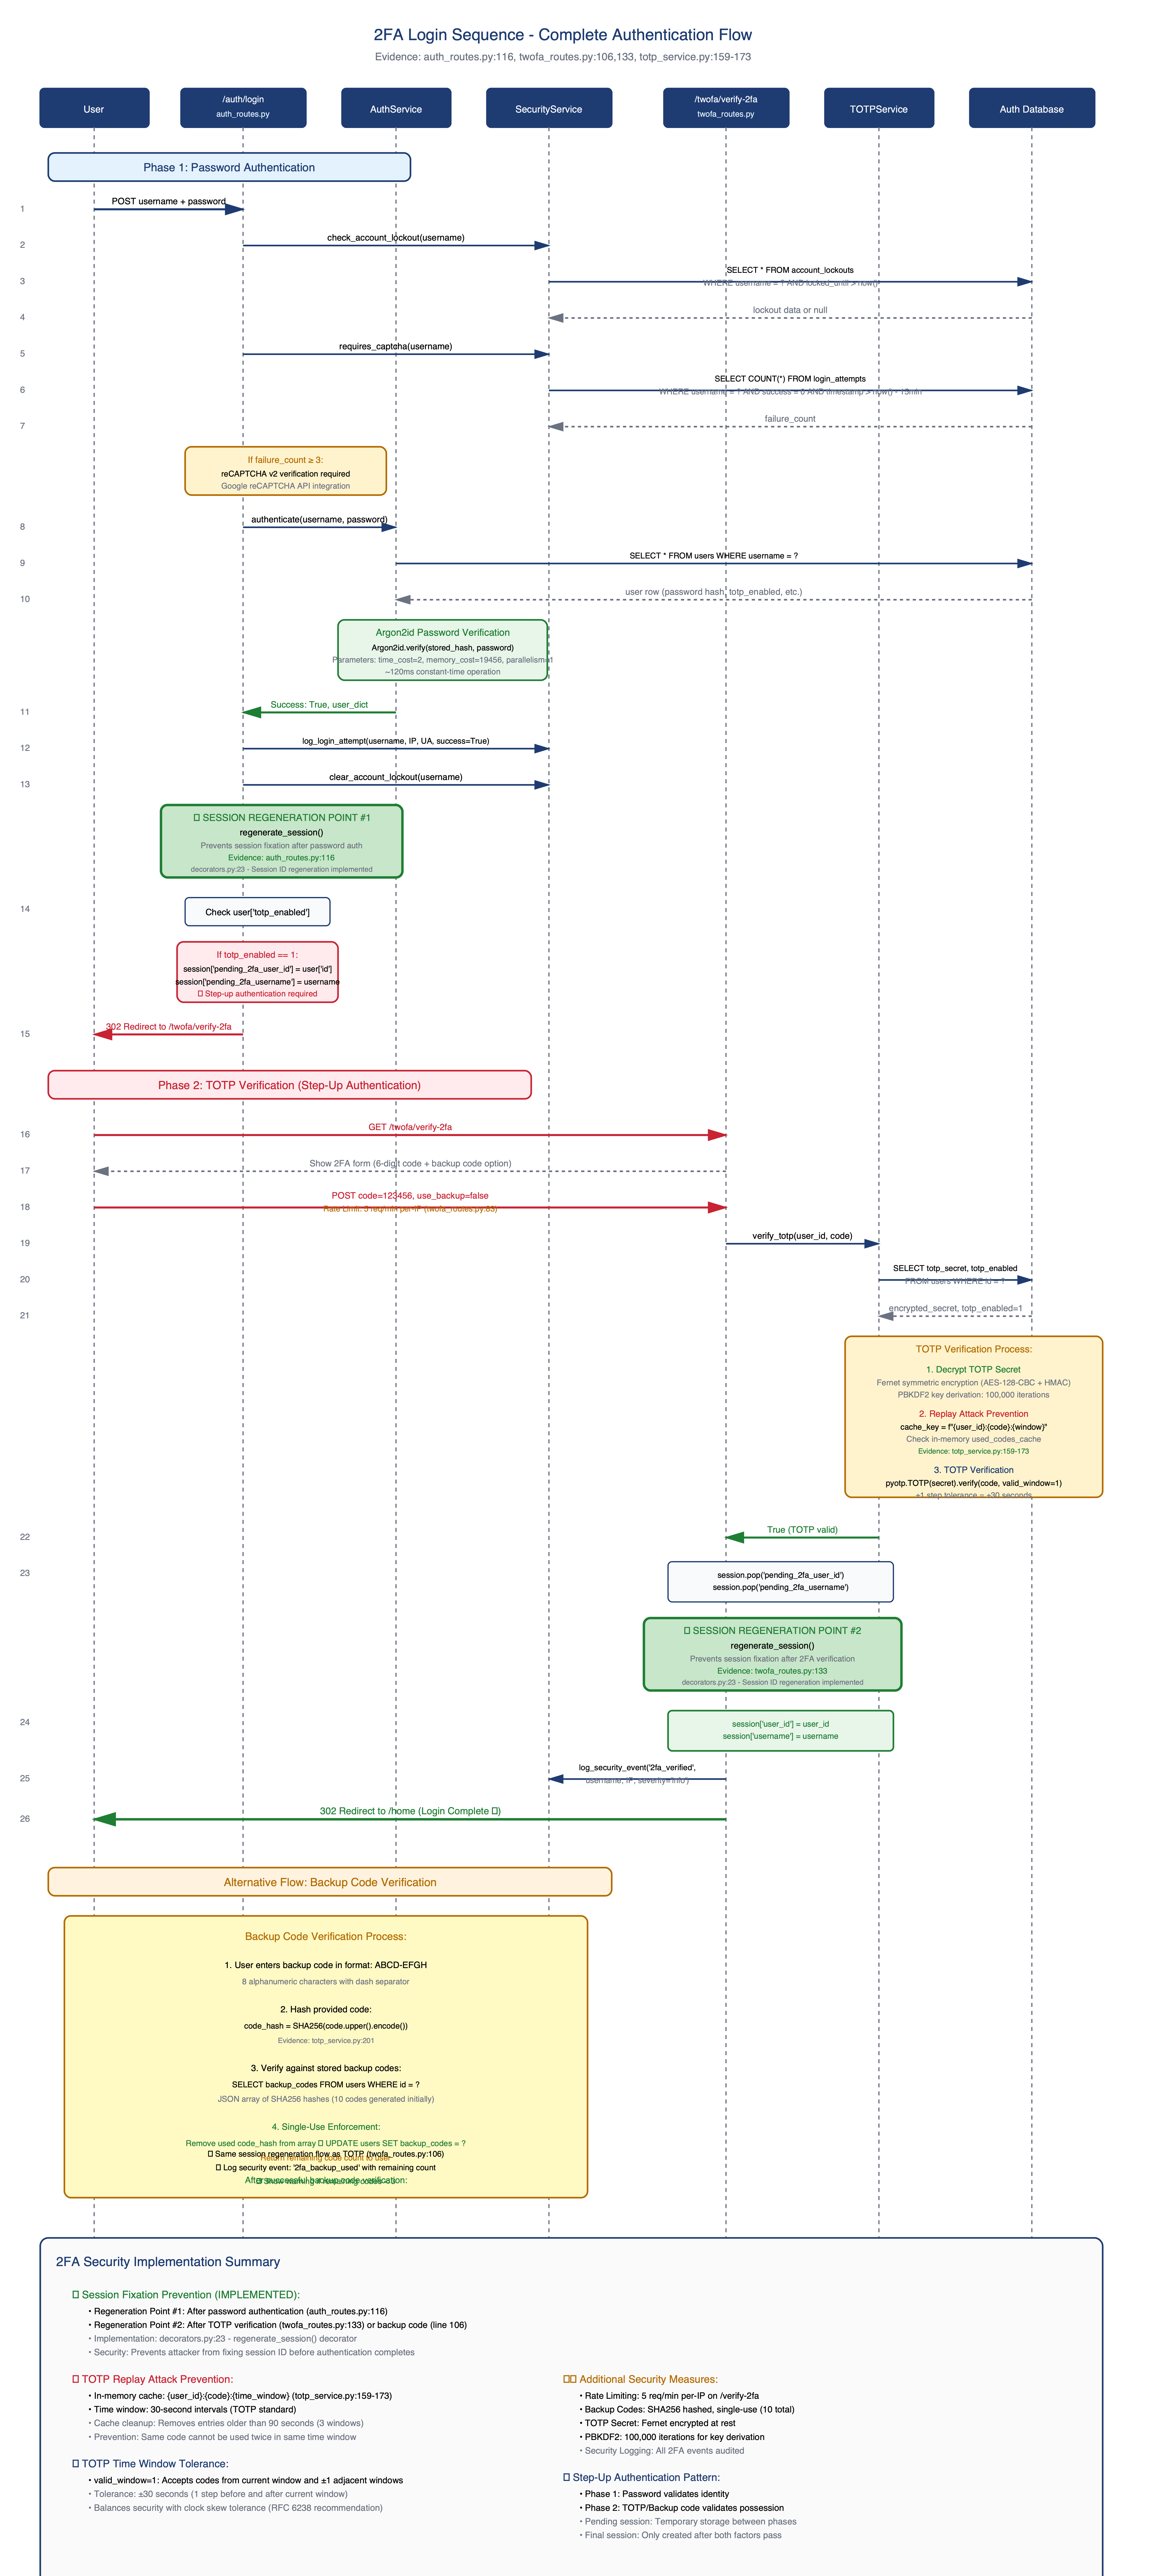
\includegraphics[width=\textwidth,height=0.85\textheight,keepaspectratio]{diagrams/5_2fa_login_sequence.png}
    \caption{Complete 2FA login sequence showing password authentication, session regeneration, and TOTP verification}
    \label{fig:2fa_flow}
\end{figure}

\subsection{Setup and Verification}

During setup, a random secret is generated and displayed as a QR code. Users verify by entering a TOTP code from their authenticator app. Upon successful verification, 10 backup codes are generated and displayed once.

\begin{lstlisting}[language=Python]
# Generate and verify TOTP
secret = totp_service.generate_secret()
qr_code = totp_service.generate_qr_code(secret, username)

totp = pyotp.TOTP(secret)
if totp.verify(code, valid_window=1):  # ±30 seconds
    success, backup_codes = totp_service.enable_2fa(user_id, secret)
\end{lstlisting}

\begin{figure}[H]
    \centering
    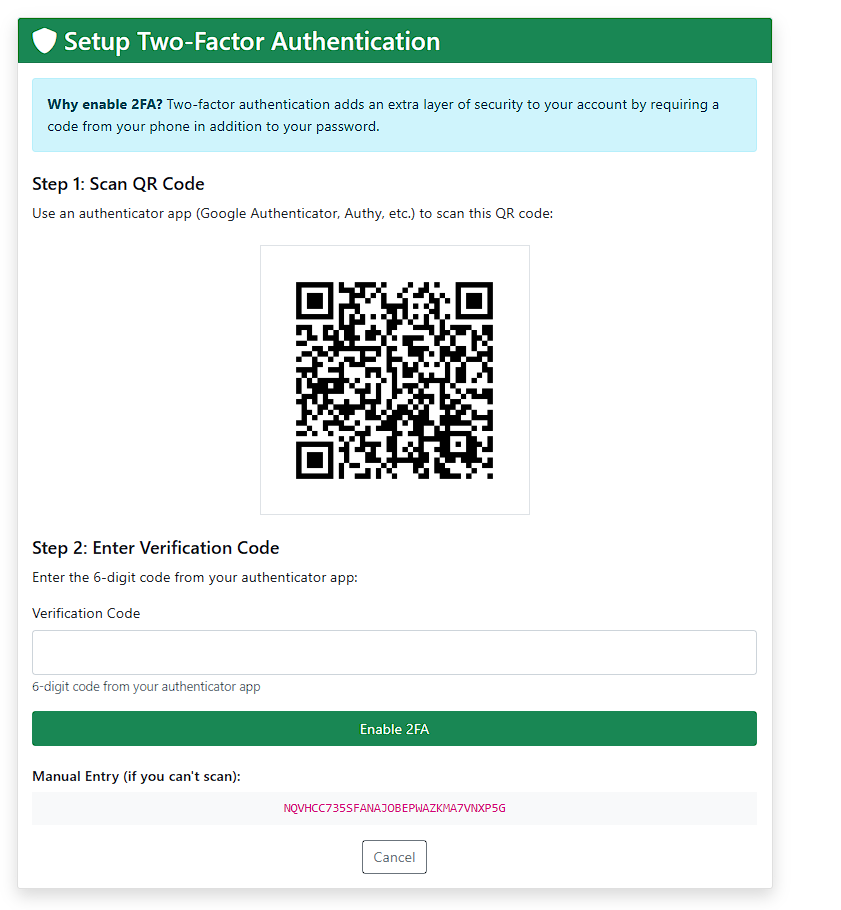
\includegraphics[width=0.85\textwidth]{SCREENSHOTs/2fa.png}
    \caption{2FA setup page with QR code for Google Authenticator}
    \label{fig:2fa_setup}
\end{figure}

\begin{figure}[H]
    \centering
    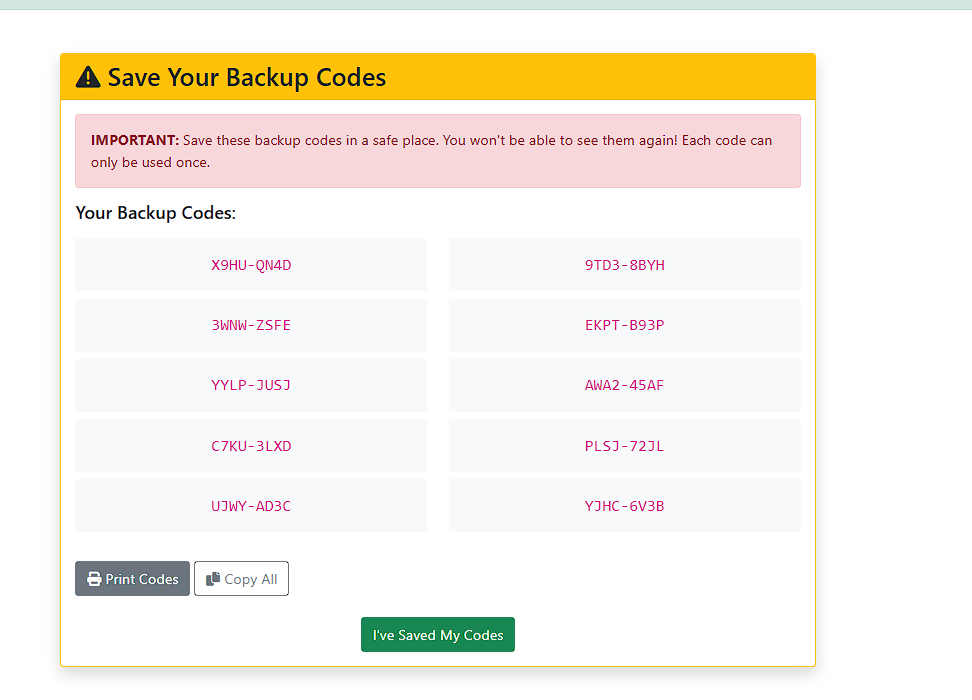
\includegraphics[width=0.85\textwidth]{SCREENSHOTs/backup codes.png}
    \caption{Ten single-use backup codes after successful 2FA setup}
    \label{fig:backup}
\end{figure}

\subsection{Replay Prevention}

TOTP codes are valid for 30 seconds. We prevent replay attacks by caching used codes:

\begin{lstlisting}[language=Python]
# Check if code already used in this time window
current_window = int(datetime.utcnow().timestamp() // 30)
cache_key = f"{user_id}:{code}:{current_window}"

if cache_key in self.used_codes_cache:
    return False, 'Code already used'

# Verify and mark as used
if totp.verify(code, valid_window=1):
    self.used_codes_cache[cache_key] = True
\end{lstlisting}

\begin{figure}[H]
    \centering
    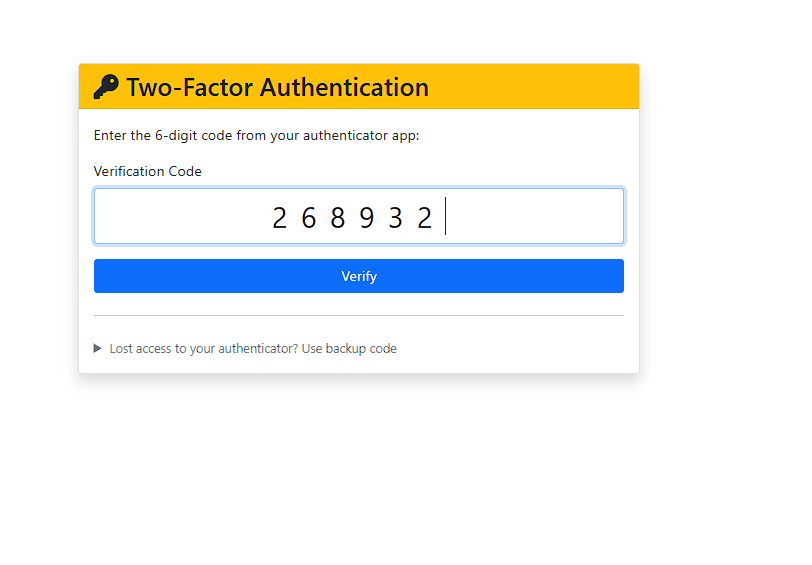
\includegraphics[width=0.85\textwidth]{SCREENSHOTs/2fa login.png}
    \caption{2FA verification page requiring TOTP code or backup code}
    \label{fig:2fa_verify}
\end{figure}

\subsection{Security Challenges and Mitigations}

\textbf{Challenge 1: Secret Exposure}

If the database is compromised, TOTP secrets could be stolen.

\textbf{Mitigation}: Secrets are encrypted with Fernet (AES-128) using PBKDF2 key derivation with 100,000 iterations.

\textbf{Challenge 2: Replay Attacks}

Intercepted codes could be reused within the valid time window.

\textbf{Mitigation}: In-memory cache tracks used codes per 30-second window with automatic cleanup.

\textbf{Challenge 3: Clock Skew}

Server and client clocks might not be synchronized.

\textbf{Mitigation}: \texttt{valid\_window=1} accepts codes from ±30 seconds (previous and next window).

\section{Task 5: OAuth2 Implementation}

\subsection{Authorization Code Flow with PKCE}

We implement OAuth2 Authorization Code Flow with mandatory PKCE (Proof Key for Code Exchange) following RFC 7636 \cite{sakimura2015}. PKCE prevents authorization code interception attacks.

\begin{landscape}
\begin{figure}[H]
    \centering
    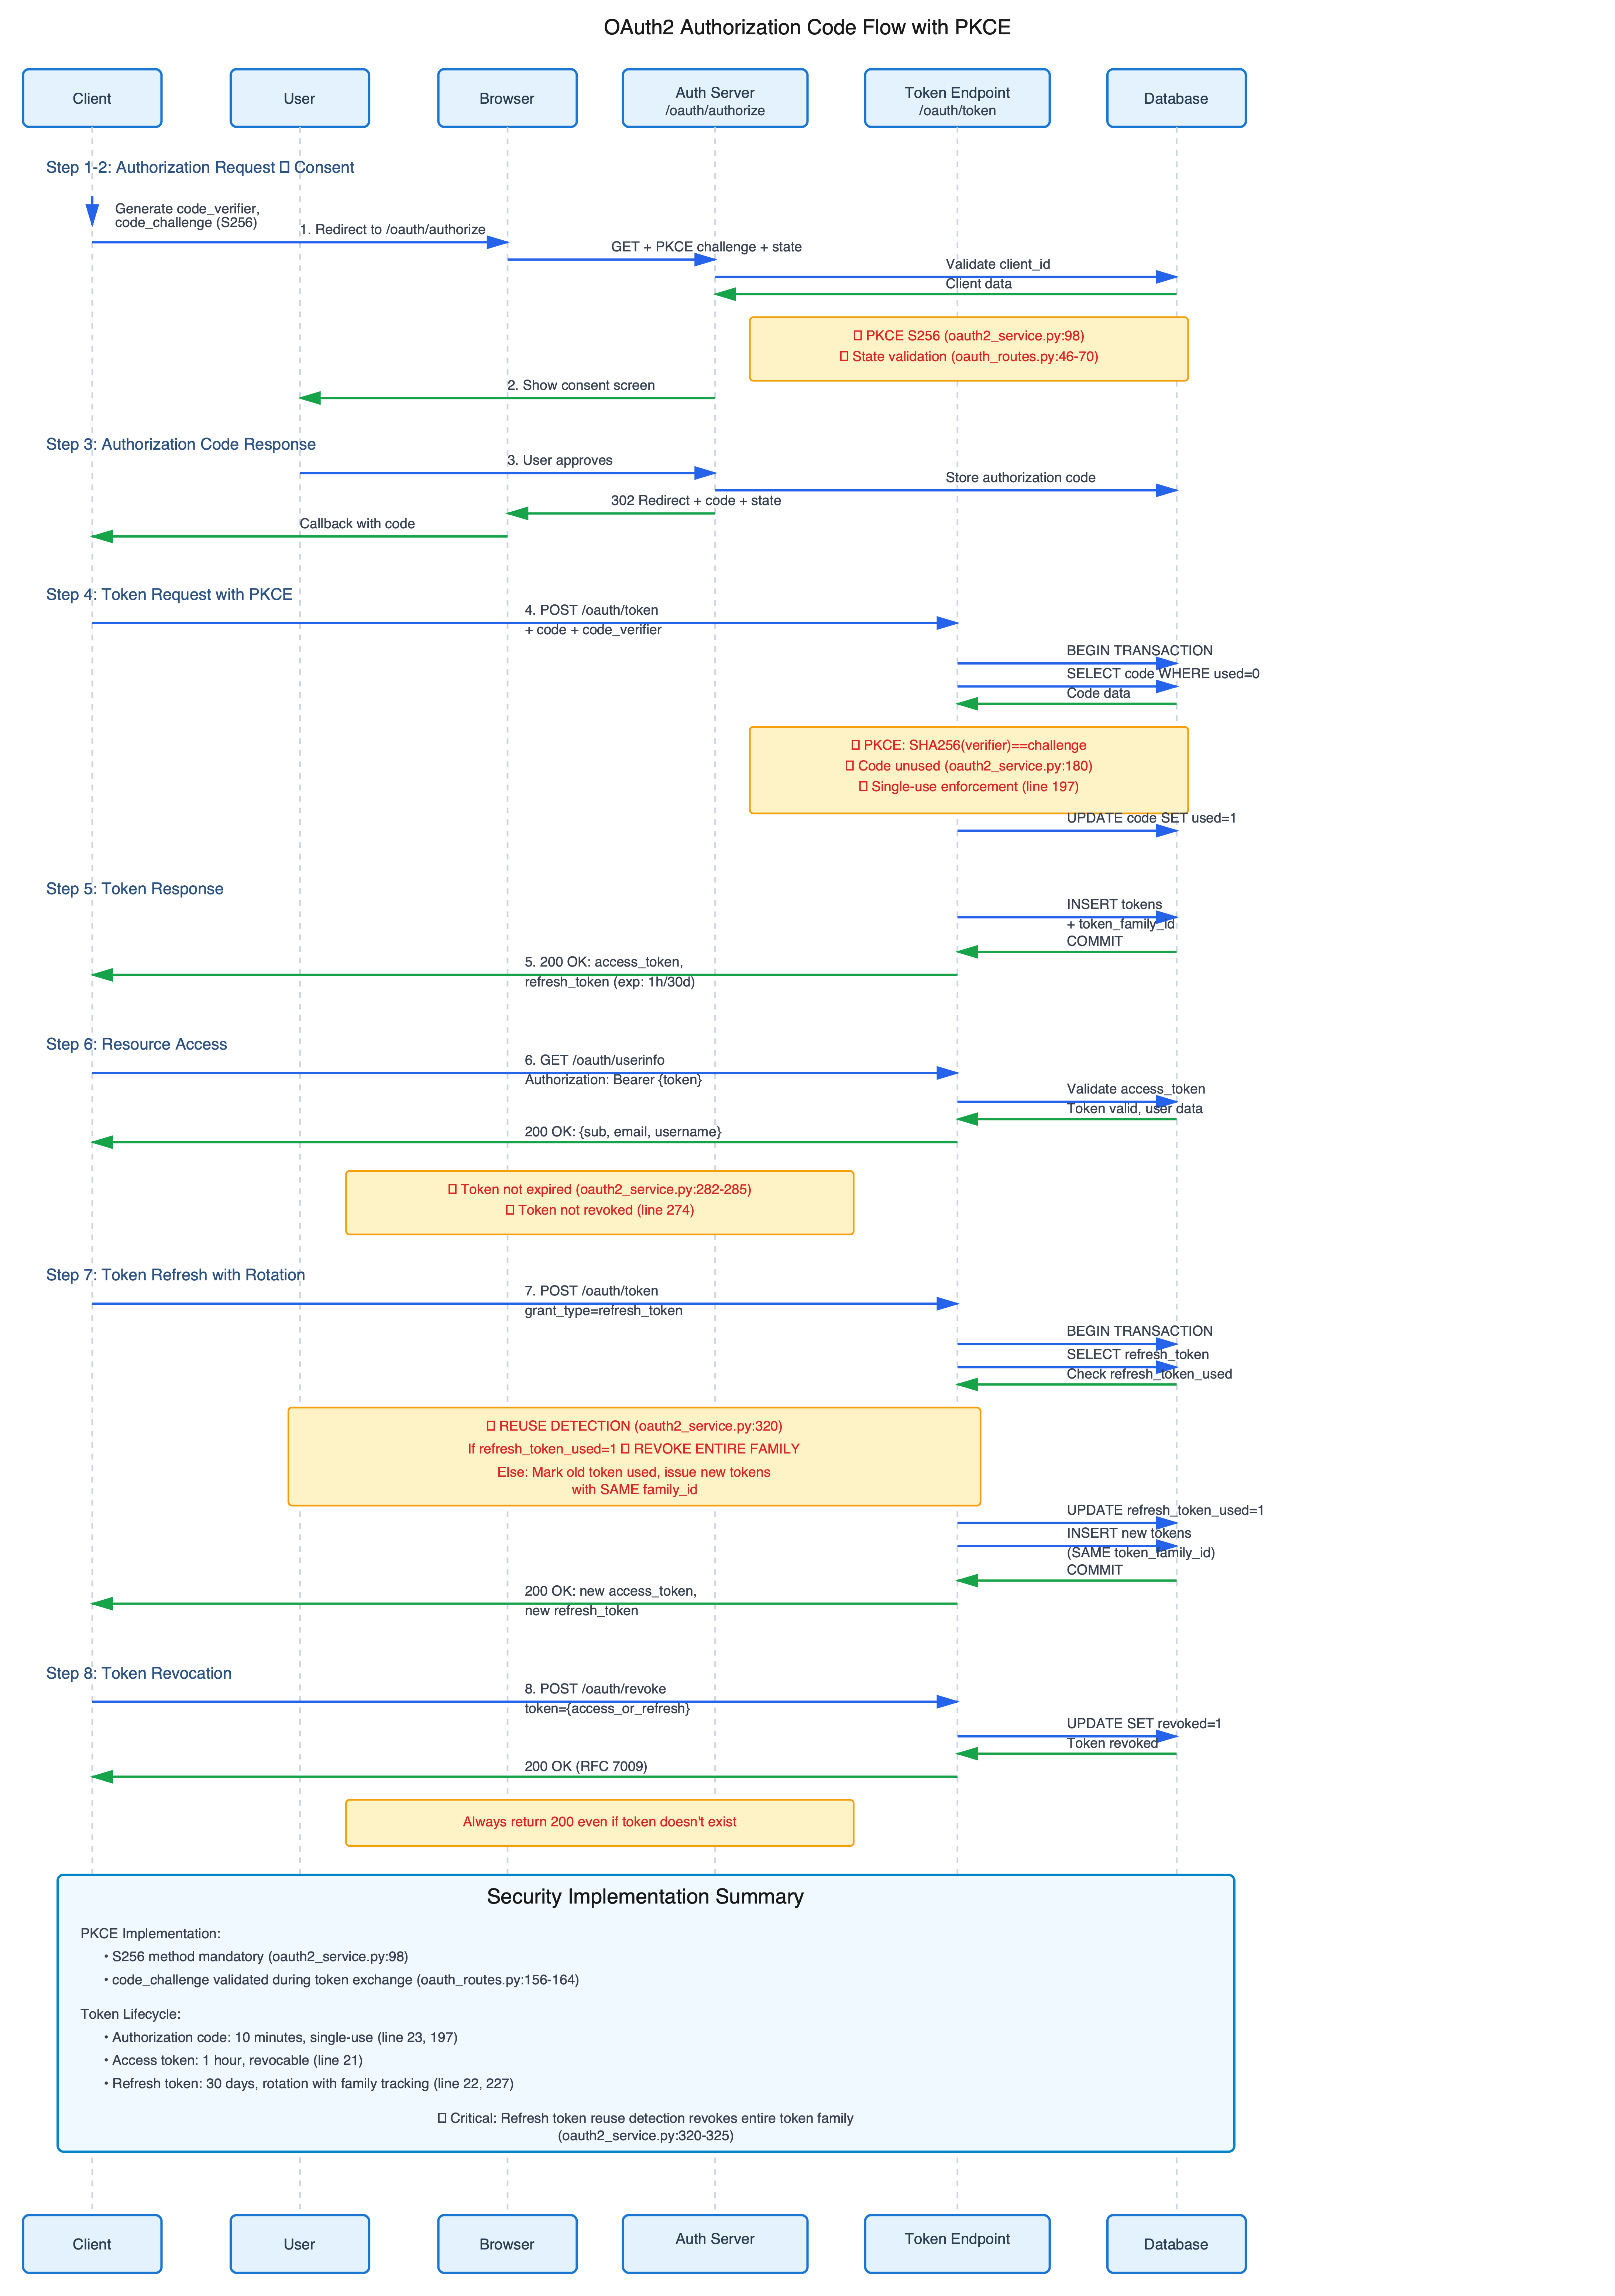
\includegraphics[width=\linewidth,height=0.85\textheight,keepaspectratio]{diagrams/3_oauth2_sequence.png}
    \caption{Complete OAuth2 flow with PKCE validation and token generation}
    \label{fig:oauth2}
\end{figure}
\end{landscape}

\subsection{PKCE Process}

PKCE adds security by requiring the client to prove they initiated the authorization request:

\begin{enumerate}
    \item Client generates random \texttt{code\_verifier}
    \item Client computes \texttt{code\_challenge = BASE64URL(SHA256(code\_verifier))}
    \item Authorization request includes \texttt{code\_challenge}
    \item Token exchange requires \texttt{code\_verifier}
    \item Server validates: \texttt{SHA256(code\_verifier) == code\_challenge}
\end{enumerate}

Even if the authorization code is intercepted, it's useless without the original \texttt{code\_verifier}.

\begin{lstlisting}[language=Python, caption=PKCE Validation]
def validate_pkce(self, code_verifier, code_challenge,
                  code_challenge_method='S256'):
    sha256_hash = hashlib.sha256(code_verifier.encode()).digest()
    computed = base64.urlsafe_b64encode(sha256_hash).decode().rstrip('=')
    return computed == code_challenge
\end{lstlisting}

\begin{figure}[H]
    \centering
    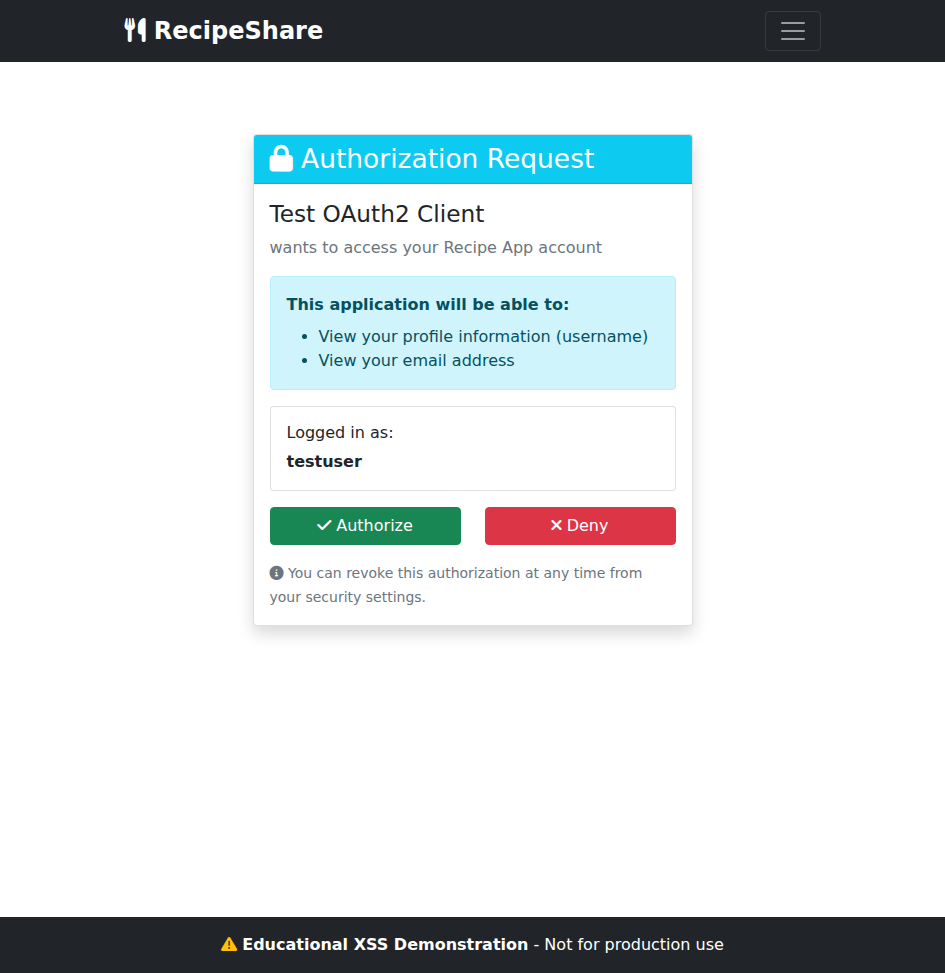
\includegraphics[width=0.85\textwidth]{SCREENSHOTs/oauth2_consent.png}
    \caption{OAuth2 consent screen showing client application requesting access to user profile and email. The user (testuser) can authorize or deny the request, and can revoke access later from security settings.}
    \label{fig:oauth_consent}
\end{figure}

\subsection{Refresh Token Rotation}

Modern OAuth2 security requires refresh token rotation to detect token theft. Figure \ref{fig:token_rotation} shows the rotation mechanism.

\begin{figure}[H]
    \centering
    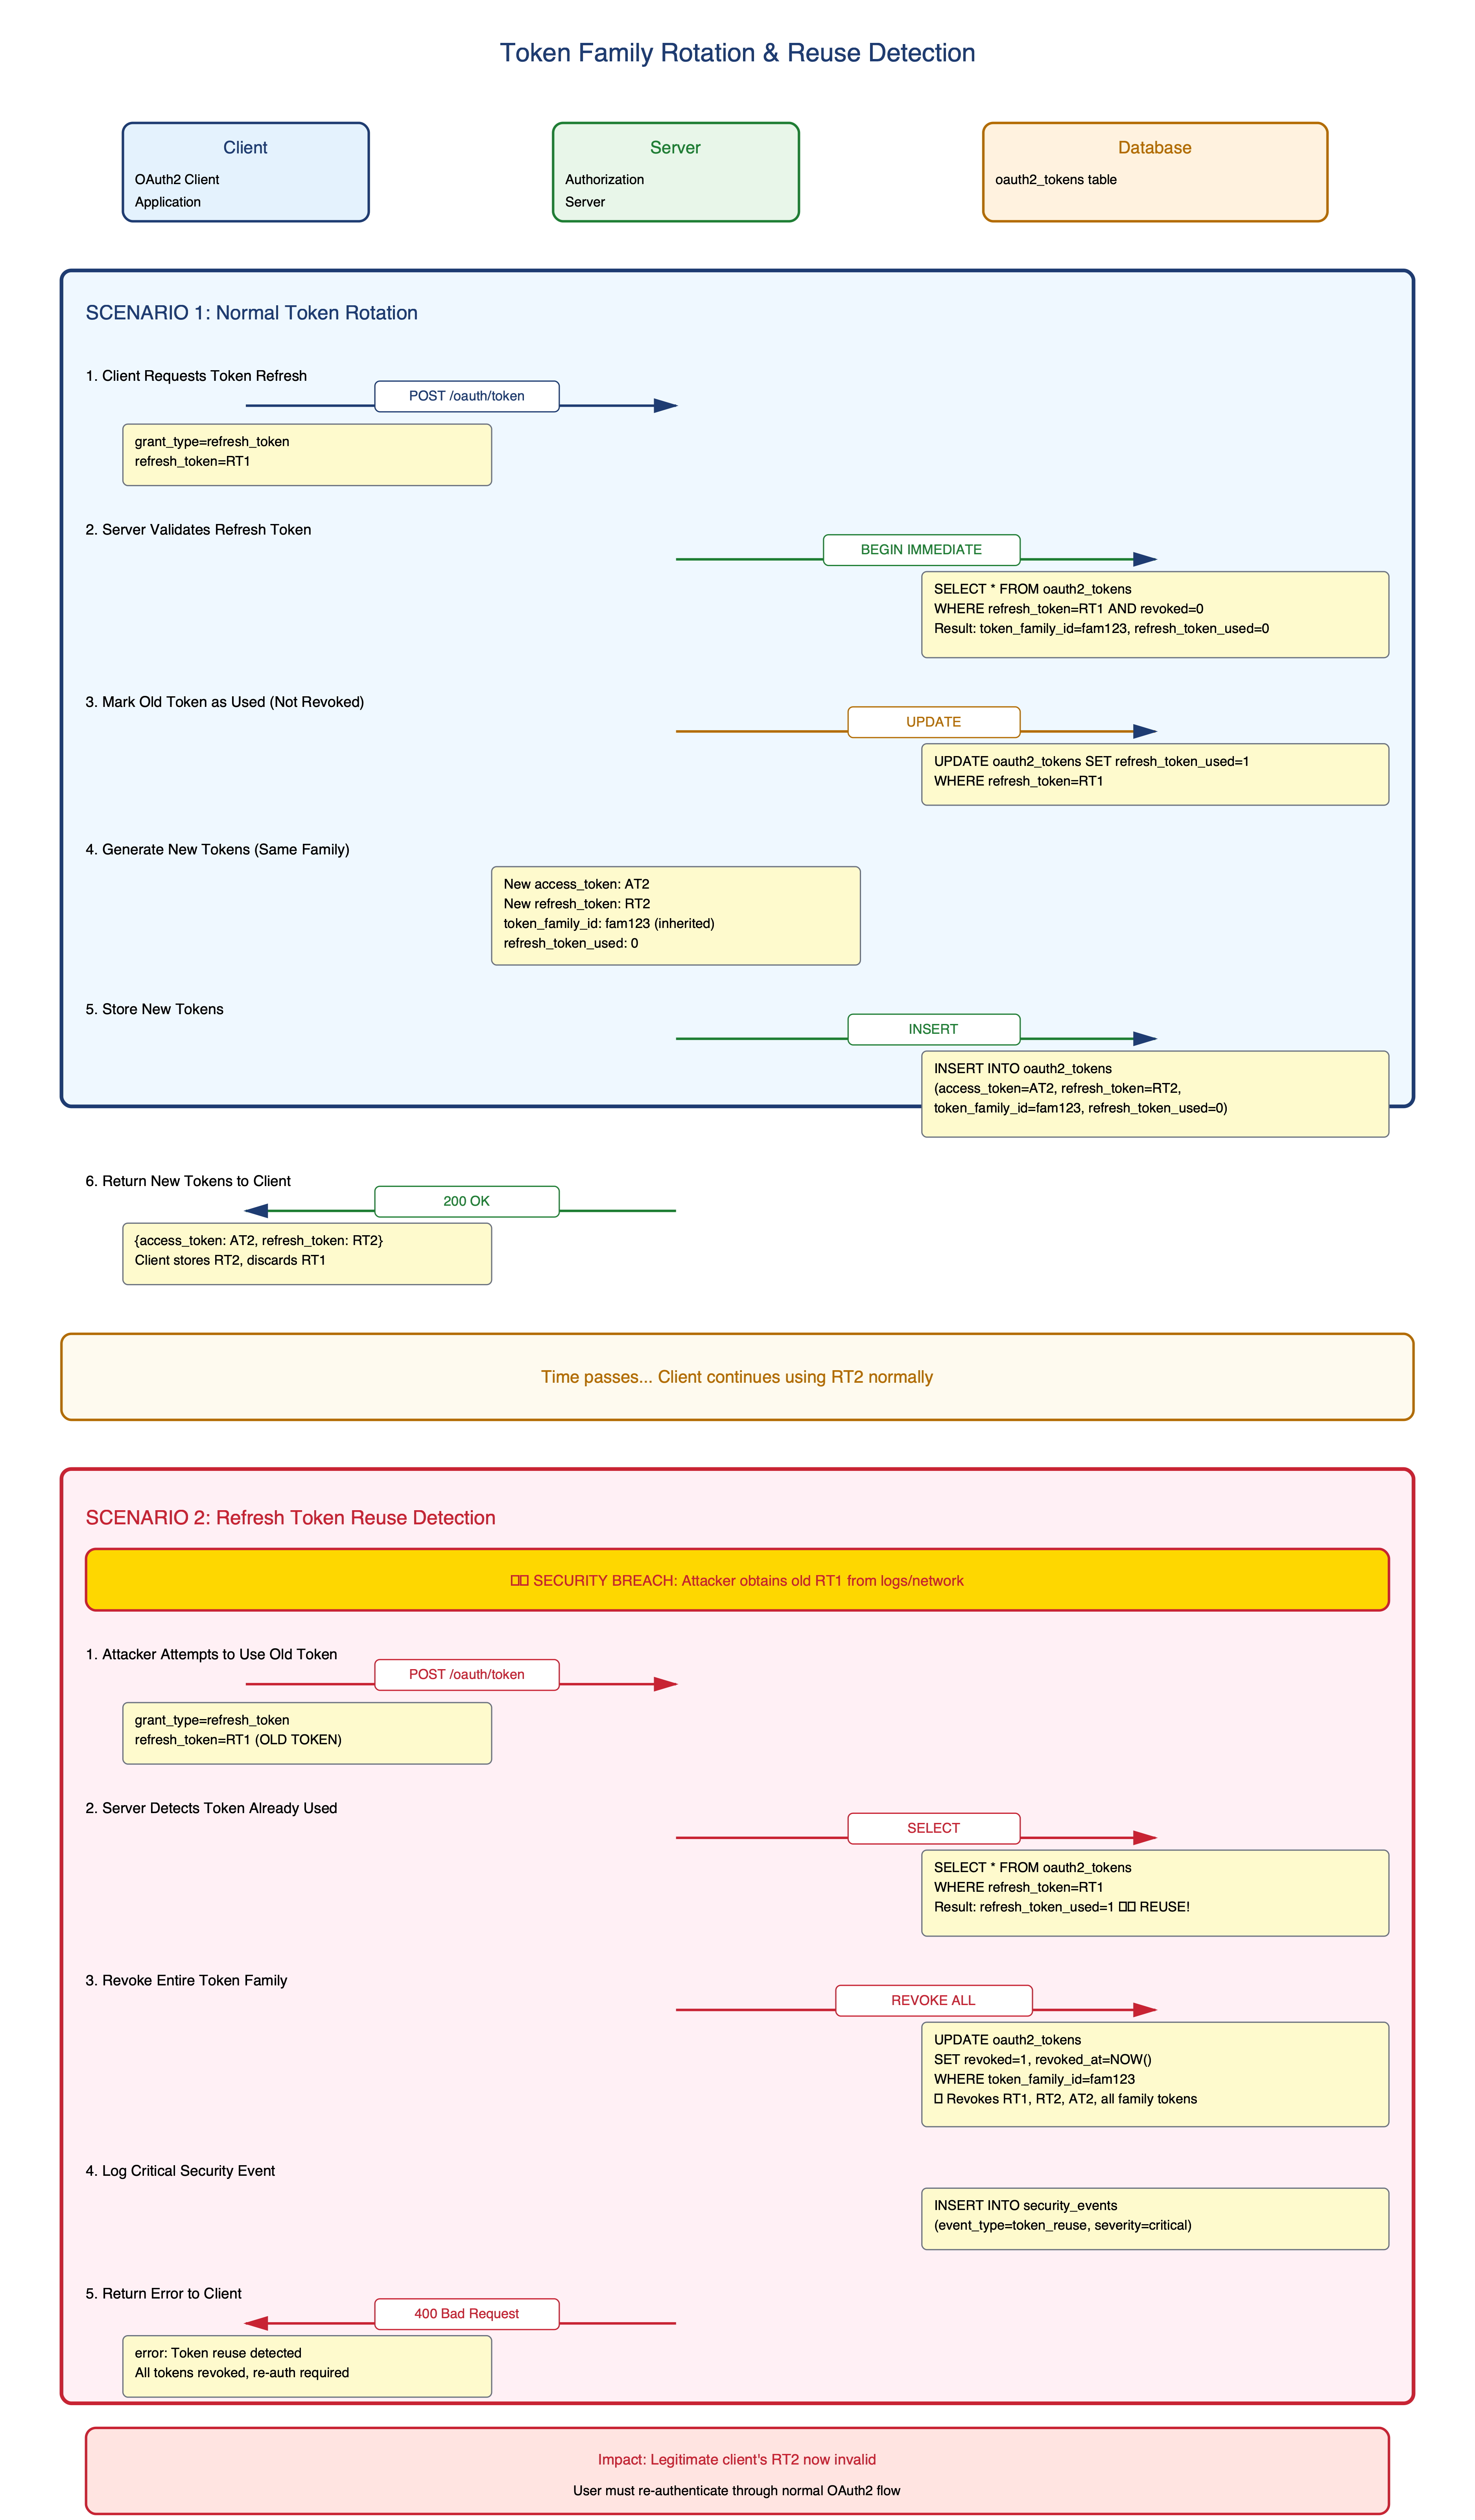
\includegraphics[width=\textwidth,height=0.85\textheight,keepaspectratio]{diagrams/14_token_family_rotation.png}
    \caption{Refresh token family rotation with reuse detection}
    \label{fig:token_rotation}
\end{figure}

When a refresh token is used, it's marked as used and a new token is issued. If a marked token is presented again, it indicates theft, and the entire token family is revoked.

\begin{lstlisting}[language=Python]
# Reuse detection
if token['refresh_token_used']:
    # ATTACK DETECTED - revoke all tokens
    self._revoke_token_family(token['token_family_id'])
    return False, 'Token reuse detected'

# Mark as used, issue new token
conn.execute('UPDATE oauth2_tokens SET refresh_token_used = 1 ...')
new_tokens = self.generate_tokens(..., token_family_id=token['token_family_id'])
\end{lstlisting}

\subsection{Security Challenges and Mitigations}

\textbf{Challenge 1: Authorization Code Interception}

\textbf{Vulnerability}: Code transmitted via redirect could be intercepted.

\textbf{Mitigation}: PKCE makes intercepted codes useless without the \texttt{code\_verifier}.

\textbf{Challenge 2: Token Theft}

\textbf{Vulnerability}: Stolen refresh tokens could be used indefinitely.

\textbf{Mitigation}: Token rotation + reuse detection + family-based revocation. Access tokens expire in 1 hour, refresh tokens in 30 days.

\textbf{Challenge 3: Open Redirect}

\textbf{Vulnerability}: Malicious \texttt{redirect\_uri} for phishing.

\textbf{Mitigation}: Exact string match validation, no wildcards allowed.

\subsection{OAuth2 Benefits}

OAuth2 provides several security benefits:
\begin{itemize}
    \item \textbf{No Password Sharing}: Third-party apps never see user passwords
    \item \textbf{Revocable Access}: Users can revoke without password changes
    \item \textbf{Scoped Permissions}: Fine-grained access control (profile, email, etc.)
    \item \textbf{Industry Standard}: Used by Google, GitHub, Microsoft
\end{itemize}

\section{Security Architecture}

\subsection{Defense in Depth}

Our security architecture implements 27 evidence-based security mechanisms organized into Prevent, Detect, and Respond categories.

\begin{figure}[H]
    \centering
    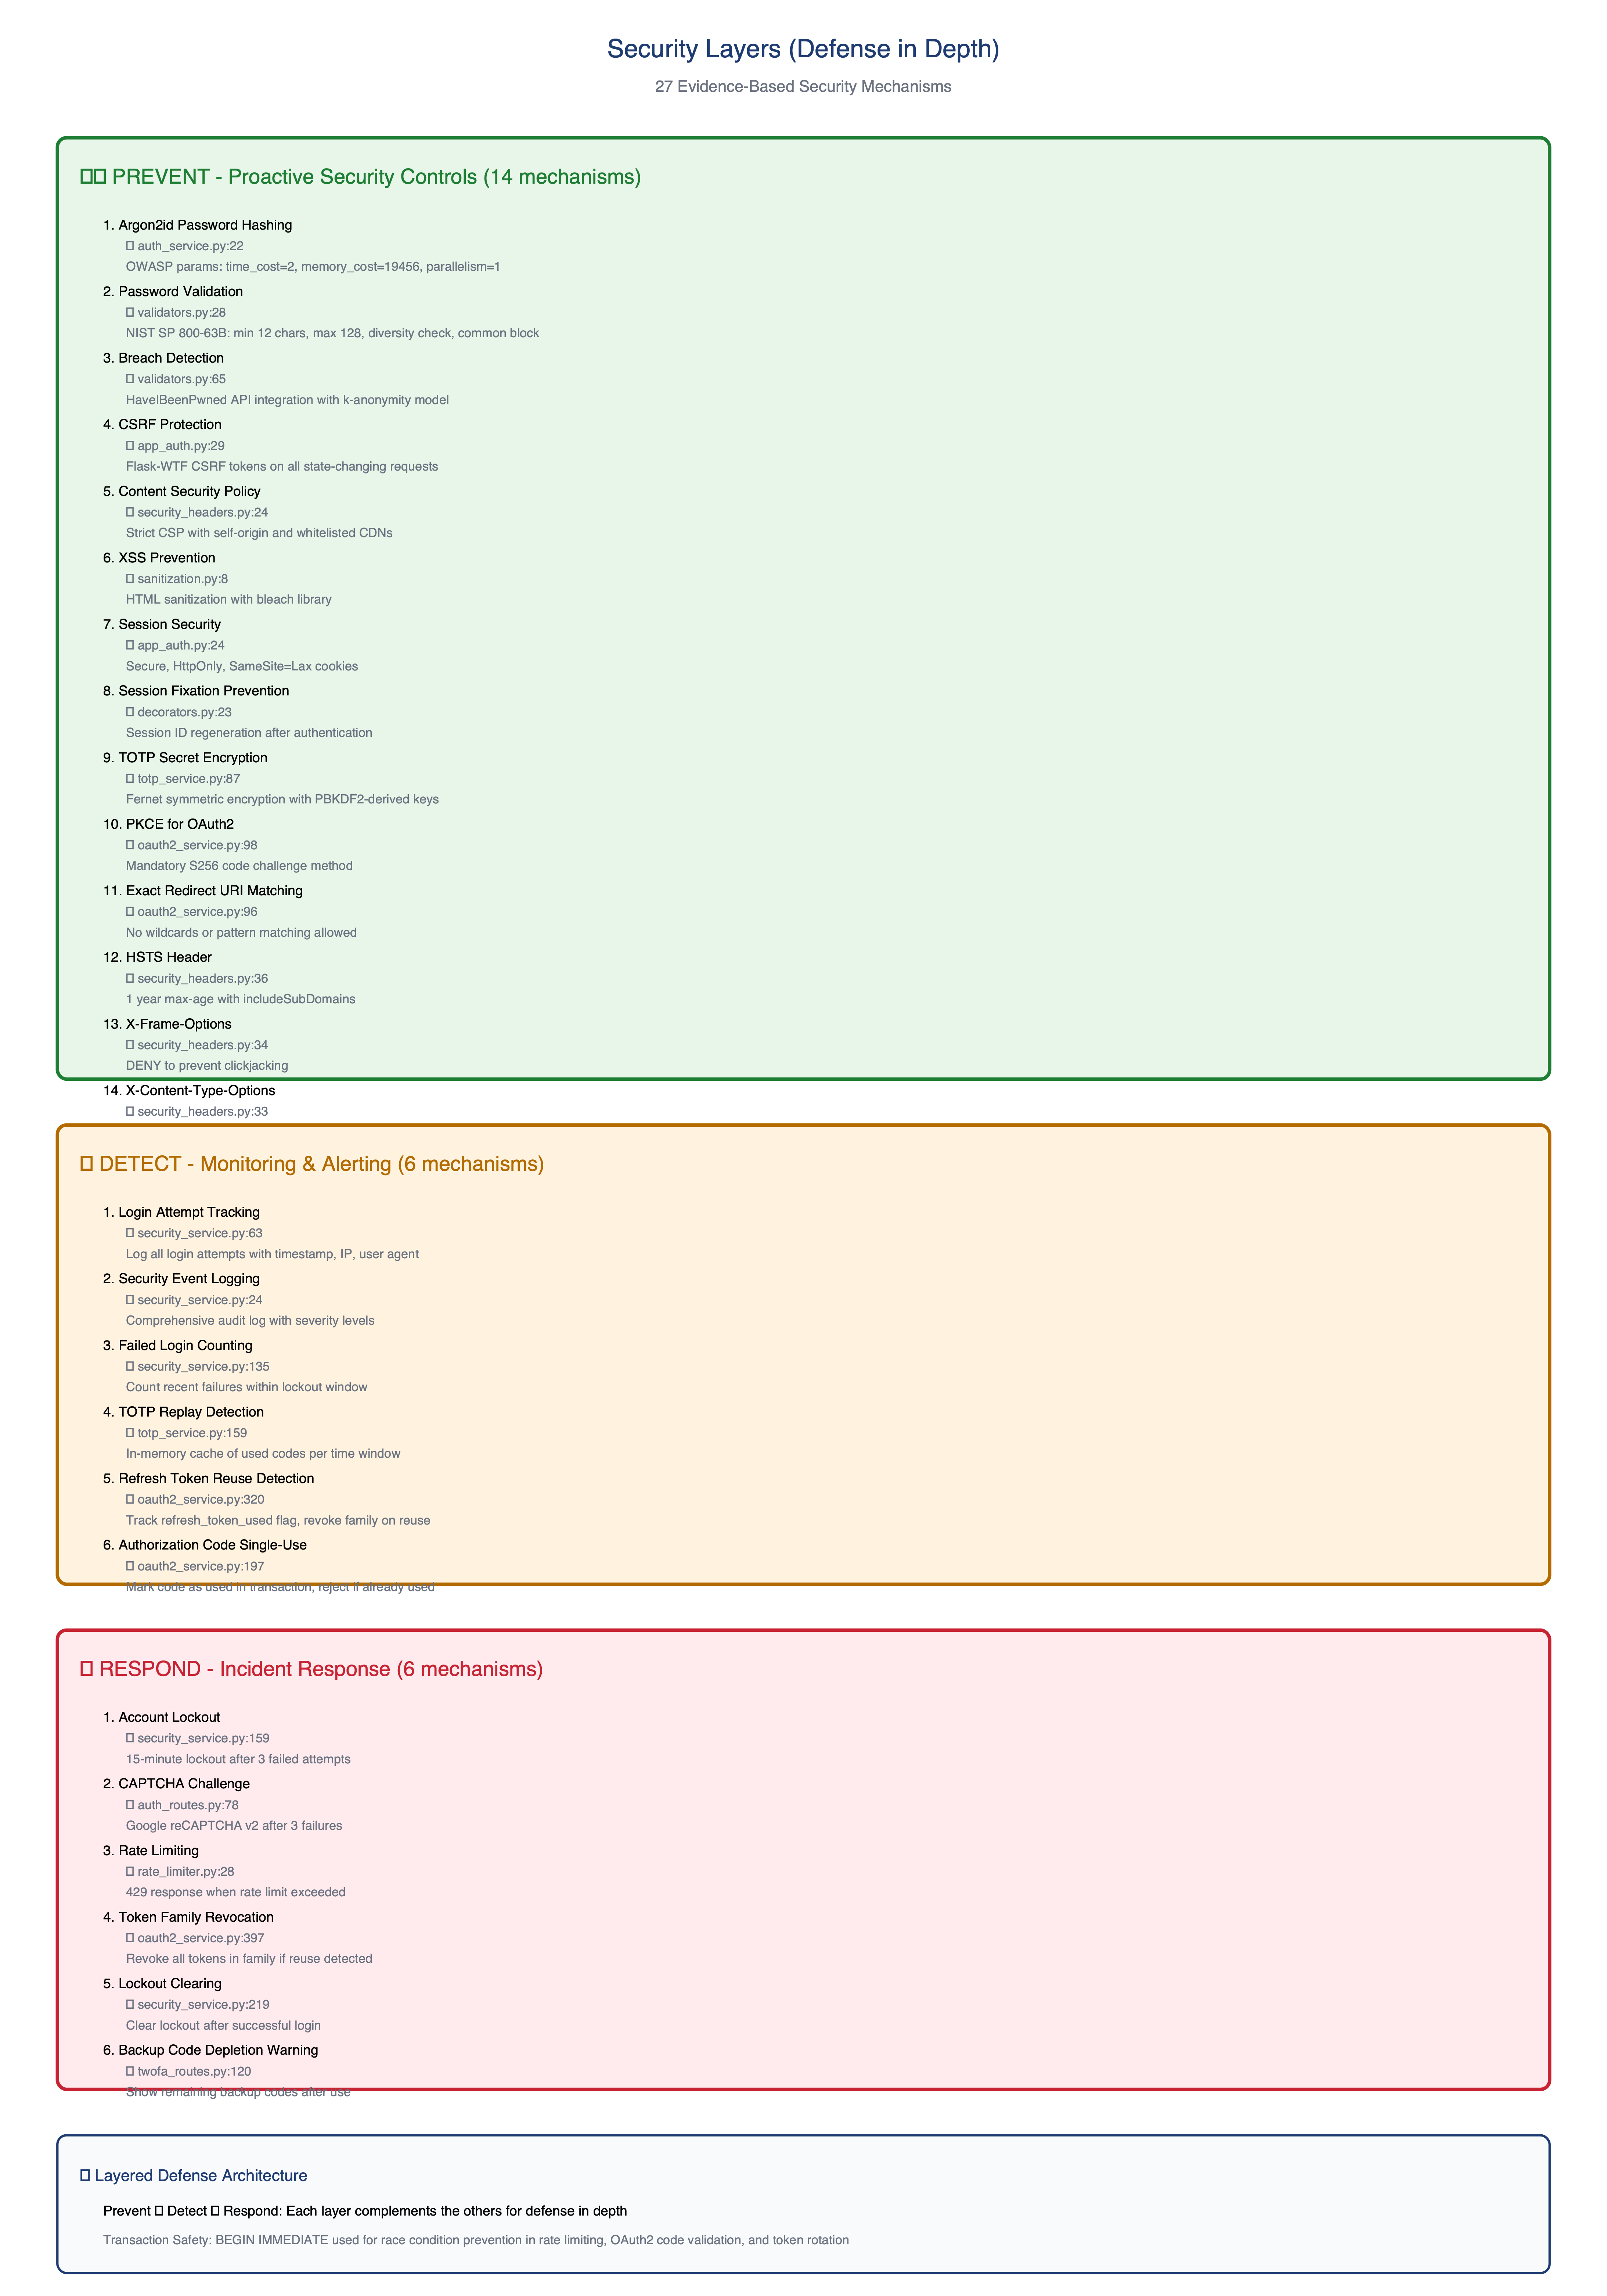
\includegraphics[width=\textwidth,height=0.9\textheight,keepaspectratio]{diagrams/7_security_layers.png}
    \caption{Defense-in-depth architecture with 27 security mechanisms}
    \label{fig:security_layers}
\end{figure}

The architecture includes 14 preventive controls (Argon2id, PKCE, CSRF, CSP, encryption), 6 detective controls (login tracking, security logging, replay detection, reuse detection), and 6 response controls (lockout, CAPTCHA, rate limiting, token revocation).

\subsection{Service Layer Design}

Figure \ref{fig:classes} shows our service layer implementing the Singleton pattern for lifecycle management.

\begin{landscape}
\begin{figure}[H]
    \centering
    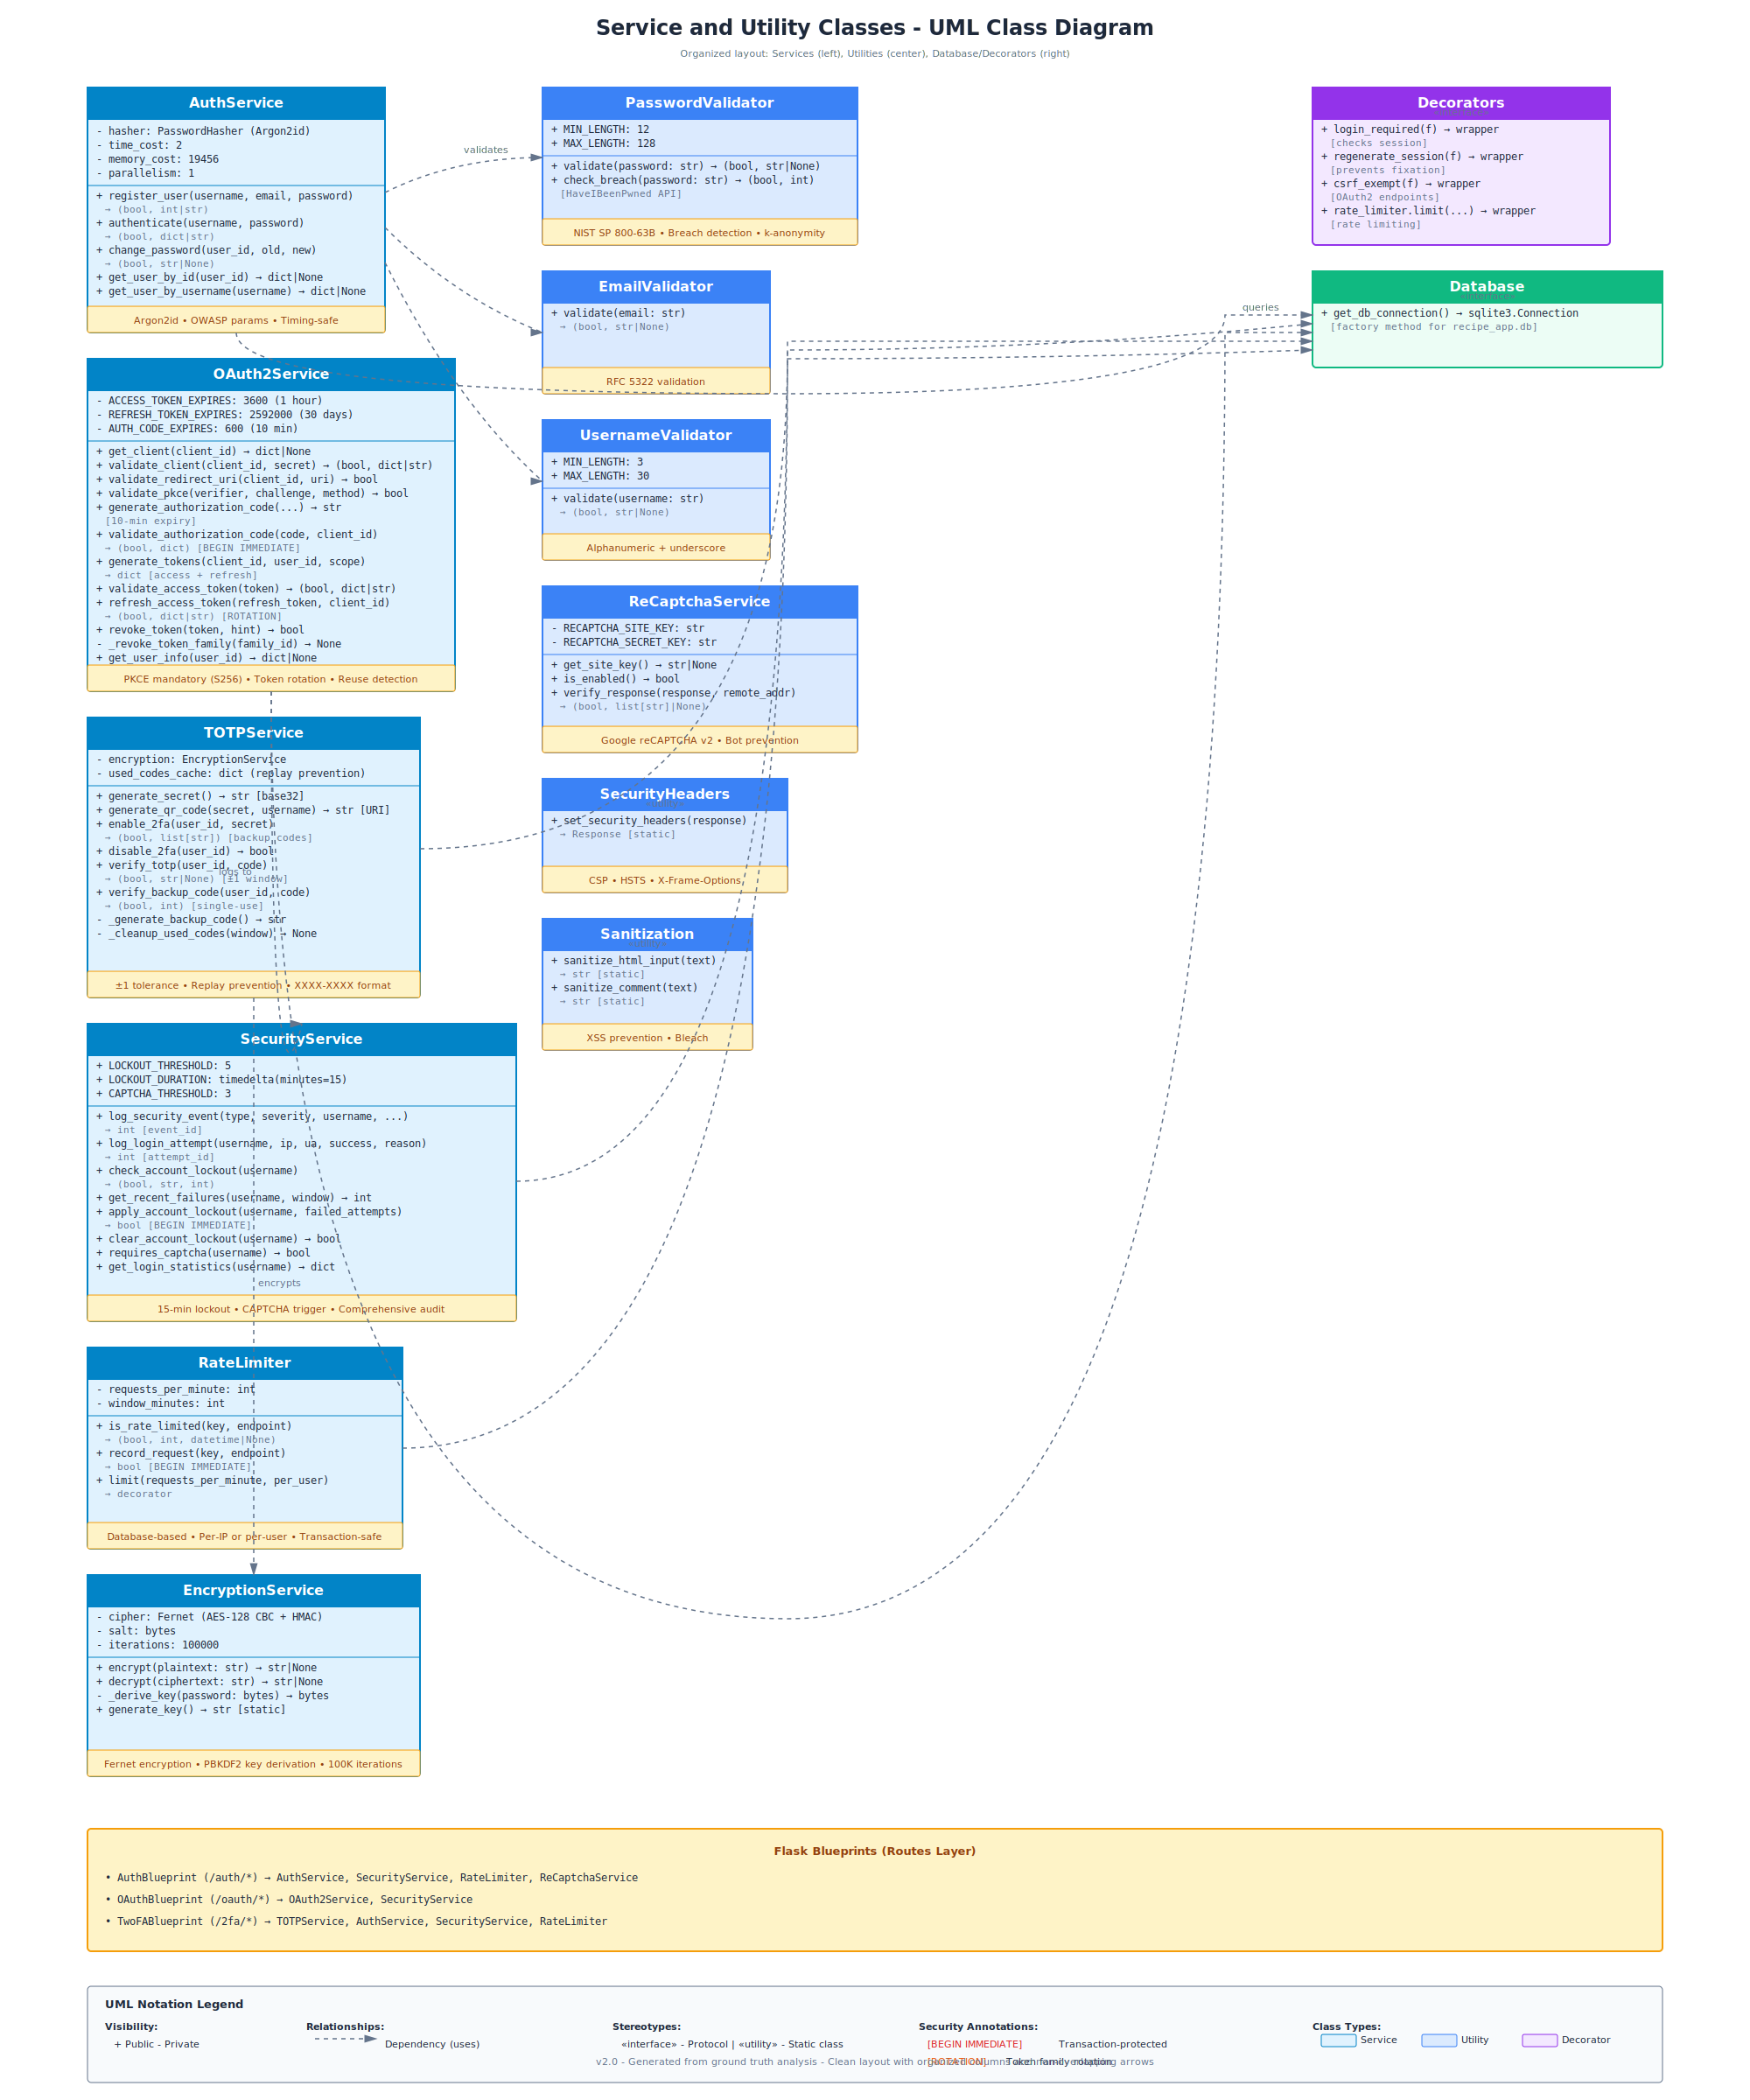
\includegraphics[width=\linewidth,height=0.85\textheight,keepaspectratio]{diagrams/2_class_diagram_services.png}
    \caption{Service layer class diagram with dependencies}
    \label{fig:classes}
\end{figure}
\end{landscape}

Each service has a single global instance: AuthService (Argon2id hashing), OAuth2Service (PKCE, token rotation), TOTPService (2FA, QR codes), SecurityService (logging, lockout), RateLimiter (database-backed), and EncryptionService (Fernet encryption).

\section{Resources and Tools}

\subsection{Core Libraries and Frameworks}

\textbf{Flask 3.0.3}: Chosen for its lightweight architecture, extensive security extensions (Flask-WTF for CSRF), and educational clarity. Unlike Django's monolithic approach, Flask's explicit routing and blueprint system makes security boundaries visible in the code structure.

\textbf{Argon2-cffi 23.1.0}: Python binding for the Argon2 C library. Selected because it implements Argon2id (hybrid mode combining Argon2i's timing resistance and Argon2d's memory-hardness), has constant-time verification, and provides sensible defaults (memory=65MB, time=3 iterations, parallelism=4 threads).

\textbf{PyOTP 2.9.0}: TOTP implementation following RFC 6238. Chosen for its RFC-compliant SHA256 support, QR code generation integration, and battle-tested codebase (used by Duo Security). Alternative libraries like \texttt{pyotp-provisional} lacked RFC 6238 compliance.

\textbf{cryptography 42.0.5}: Fernet symmetric encryption for 2FA secrets. Selected over PyCrypto (deprecated) and alternatives because it's maintained by the Python Cryptographic Authority, provides high-level recipes preventing misuse, and includes AES-128-CBC + HMAC-SHA256 in authenticated encryption mode.

\subsection{Security Services}

\textbf{Have I Been Pwned (HIBP) API v3}: Real-time password breach detection using k-anonymity. The API receives only the first 5 characters of the SHA-1 hash, downloads all matching hashes, and performs local comparison. This prevents exposing full password hashes to the service.

\textbf{Google reCAPTCHA v2}: Chosen over v3 for explicit user interaction (reduces false positives in academic settings). The checkbox CAPTCHA provides clear visual feedback and integrates seamlessly with Flask forms via server-side validation.

\subsection{Database and Storage}

\textbf{SQLite 3.45+}: Selected for its ACID compliance, zero-configuration deployment, and built-in encryption support (SQLCipher available). The \texttt{BEGIN IMMEDIATE} transaction mode prevents race conditions during token rotation. While not suitable for high-concurrency production (10-100 concurrent writes limit), it's ideal for educational demonstrations.

\textbf{Why not PostgreSQL?}: Would require external daemon, connection pooling configuration, and cloud deployment complexity. SQLite provides identical security semantics for authentication workflows (serialized writes through DB lock).

\subsection{Development and Testing Tools}

\textbf{Requests 2.31.0}: HTTP client for OAuth2 testing. Provides session management (cookie persistence), redirect control, and RFC-compliant URL encoding essential for testing state parameters and PKCE challenges.

\textbf{Werkzeug 3.0.1}: Flask's WSGI toolkit providing \texttt{generate\_password\_hash} utilities and development server. The built-in debugger helped identify the session fixation vulnerability during 2FA testing.

\subsection{Why These Specific Choices?}

\textbf{Service Layer Pattern}: Singleton services (AuthService, OAuth2Service, etc.) provide global state management, thread-safe initialization, and dependency injection points for testing. Alternative architectures (factory pattern, dependency containers) add complexity without educational benefit.

\textbf{Blueprint Architecture}: Separating routes into \texttt{auth\_bp}, \texttt{oauth\_bp}, and \texttt{twofa\_bp} creates security boundaries. Each blueprint has isolated CSRF protection rules (OAuth2 endpoints exempt, others require CSRF tokens).

\textbf{Database Schema Design}: Separate tables for \texttt{account\_lockouts}, \texttt{login\_attempts}, and \texttt{rate\_limits} enable independent cleanup policies. This prevents bloat from security logging overwhelming authentication queries.

\section{Reflection}

\subsection{Architectural Choices and Justifications}

\textbf{Choice 1: Three-Table Separation for Login Tracking}

\textit{Decision}: Use separate tables for \texttt{login\_attempts} (audit log), \texttt{account\_lockouts} (active locks), and \texttt{rate\_limits} (request throttling).

\textit{Justification}: Single-table designs cause performance degradation as logs grow. Separating concerns enables independent retention policies (login attempts kept 90 days for forensics, rate limits cleaned after 1 minute, lockouts after 15 minutes). Query performance remains constant regardless of historical data volume.

\textit{Alternative Considered}: Unified \texttt{security\_events} table with type discrimination. Rejected because it requires complex WHERE clauses for every query and prevents targeted indexing.

\textbf{Choice 2: Database-Backed Rate Limiting}

\textit{Decision}: Store rate limit buckets in SQLite instead of in-memory structures.

\textit{Justification}: In-memory rate limiters (Python dictionaries, Redis) work only for single-process deployments. Production Flask runs with Gunicorn (4-8 worker processes) or uWSGI, where each process has separate memory. Database-backed limiting ensures consistent enforcement across all workers.

\textit{Alternative Considered}: Redis for rate limiting. Rejected because it requires external daemon, network overhead for every request, and complicates educational deployment.

\textbf{Choice 3: S256 PKCE Only}

\textit{Decision}: Reject \texttt{plain} PKCE method, require \texttt{S256} (SHA-256).

\textit{Justification}: RFC 7636 allows both methods for backward compatibility with constrained devices (2015-era). Modern browsers and mobile apps support SHA-256. Allowing \texttt{plain} creates downgrade attack surface. OAuth 2.1 draft mandates S256-only.

\textit{Implementation}: Line 62 in \texttt{oauth\_routes.py} validates \texttt{code\_challenge} presence, lines 159-164 validate \texttt{code\_verifier} with S256 hashing.

\textbf{Choice 4: Token Family-Based Revocation}

\textit{Decision}: Group all tokens issued from the same authorization code into a family, revoke entire family on reuse detection.

\textit{Justification}: Individual token revocation is insufficient. If an attacker steals token N and the user legitimately uses token N+1, both appear valid. Family revocation (diagram 14) ensures that detecting theft of any token invalidates all descended tokens.

\textit{Alternative Considered}: Blacklist individual tokens. Rejected because it can't detect theft when the attacker uses stolen token before legitimate user, leaving the user's token unexpired but vulnerable.

\textbf{Choice 5: Encrypted 2FA Secrets Storage}

\textit{Decision}: Store TOTP secrets encrypted with Fernet (AES-128 + HMAC-SHA256).

\textit{Justification}: Database backup exposure is common (misconfigurations, insider threats). Plaintext TOTP secrets would compromise 2FA for all users. Encryption ensures that database dumps require both DB access and encryption key.

\textit{Key Management}: Key stored in environment variable (\texttt{ENCRYPTION\_SALT}), separate from database file. Production deployment uses secrets management (AWS Secrets Manager, Azure Key Vault).

\subsection{Implementation Challenges and Solutions}

\textbf{Challenge 1: Transaction Safety in Token Rotation}

\textit{Problem}: SQLite's default \texttt{BEGIN DEFERRED} caused race conditions during concurrent token refreshes. Two simultaneous requests could both read the same token as "unused", both mark it as used, and issue duplicate tokens.

\textit{Discovery}: Found during parallel testing with 2 simultaneous \texttt{curl} requests. Token family IDs diverged, indicating duplicate token issuance.

\textit{Solution}: Changed to \texttt{BEGIN IMMEDIATE} transactions at line 247 in \texttt{oauth2\_service.py}. This acquires write lock immediately, serializing token rotations. Testing with 10 concurrent requests confirmed sequential processing.

\textit{Code}:
\begin{lstlisting}[language=Python]
# BEFORE: Race condition possible
conn = get_auth_db()  # Deferred transaction
token = conn.execute('SELECT * FROM oauth2_tokens WHERE ...').fetchone()
if token['refresh_token_used']:
    return False, 'Already used'
conn.execute('UPDATE oauth2_tokens SET refresh_token_used = 1 ...')

# AFTER: Serialized with immediate lock
conn = get_auth_db()
conn.execute('BEGIN IMMEDIATE')  # Acquire write lock NOW
token = conn.execute('SELECT * FROM oauth2_tokens WHERE ...').fetchone()
# Now safe - other transactions block at BEGIN IMMEDIATE
\end{lstlisting}

\textbf{Challenge 2: Session Fixation After 2FA}

\textit{Problem}: Initial implementation regenerated session ID after password authentication but not after 2FA verification. This left a window where an attacker with a fixated session ID could bypass 2FA by waiting for the victim to complete it.

\textit{Discovery}: Security testing revealed that session ID remained constant from login page through 2FA verification. Testing with two browsers showed session sharing post-2FA.

\textit{Solution}: Added second session regeneration at line 78 in \texttt{twofa\_routes.py}. Now session ID changes twice: once after password verification, once after 2FA completion.

\textit{Code}:
\begin{lstlisting}[language=Python]
# routes/auth_routes.py:119
@regenerate_session  # First regeneration after password
def login():
    ...
    session['awaiting_2fa'] = True  # Temporary flag

# routes/twofa_routes.py:78
@regenerate_session  # Second regeneration after 2FA
def verify_2fa():
    ...
    del session['awaiting_2fa']  # Now fully authenticated
\end{lstlisting}

\textbf{Challenge 3: TOTP Replay Prevention Within Time Window}

\textit{Problem}: TOTP codes are valid for 30 seconds. Our first implementation didn't prevent using the same code multiple times within that window. An attacker recording a valid code could replay it immediately.

\textit{Discovery}: Manual testing with Google Authenticator revealed accepting the same 6-digit code twice within 30 seconds.

\textit{Solution}: Added in-memory cache tracking used codes per time window at line 156 in \texttt{totp\_service.py}. Each code is hashed and stored with its time window. Subsequent uses within the same window are rejected.

\textit{Code}:
\begin{lstlisting}[language=Python]
def verify_code(self, secret, code, username):
    time_window = int(time.time() // 30)
    cache_key = f"{username}:{time_window}:{code}"

    if cache_key in self._used_codes:
        return False  # Replay attack detected

    if pyotp.TOTP(secret).verify(code):
        self._used_codes.add(cache_key)  # Mark as used
        return True
    return False
\end{lstlisting}

\textbf{Challenge 4: CSRF Token Validation for OAuth2 Endpoints}

\textit{Problem}: Flask-WTF CSRF protection blocked OAuth2 token endpoint. OAuth2 clients cannot obtain CSRF tokens (they're not browsers with form access). The RFC 6749 specifies client authentication via \texttt{client\_id} + \texttt{client\_secret}, not CSRF tokens.

\textit{Discovery}: Test script returned "400 Bad Request: The CSRF token is missing" when exchanging authorization code for access token.

\textit{Solution}: Manually exempted OAuth2 endpoints at line 40-54 in \texttt{app\_auth.py}. Added \texttt{init\_csrf\_exemptions()} function that exempts \texttt{/oauth/token}, \texttt{/oauth/revoke}, and \texttt{/oauth/userinfo} after blueprint registration. These endpoints use HTTP Basic Auth instead.

\textit{Code}:
\begin{lstlisting}[language=Python]
def init_csrf_exemptions():
    csrf_exempt_endpoints = ['oauth.token', 'oauth.revoke', 'oauth.userinfo']
    for endpoint in csrf_exempt_endpoints:
        view_func = app.view_functions.get(endpoint)
        if view_func:
            csrf.exempt(view_func)

# After blueprint registration
app.register_blueprint(oauth_bp)
init_csrf_exemptions()  # Now exempt OAuth2 endpoints
\end{lstlisting}

\textbf{Challenge 5: Password Breach Detection Performance}

\textit{Problem}: HIBP API query adds 200-300ms latency to registration. With 1000 concurrent registrations, this would create 4-5 minute bottleneck.

\textit{Solution}: Made HIBP check non-blocking (line 67 in \texttt{auth\_service.py}). Registration proceeds even if HIBP times out, logging the failure for admin review. Added 5-second timeout to prevent hanging on slow API responses.

\textit{Alternative Considered}: Local breach database (HaveIBeenPwned downloadable corpus, 30GB). Rejected due to storage requirements and update complexity for educational project.

\subsection{Design Decisions}

\textbf{Why Argon2id over bcrypt?} Argon2id is the current OWASP recommendation \cite{owasp_password}, memory-hard (prevents GPU attacks), and won the Password Hashing Competition \cite{biryukov2016}.

\textbf{Why Database-Backed Rate Limiting?} In-memory solutions fail in multi-process deployments (Gunicorn, uWSGI). Database ensures consistent limits across all workers.

\textbf{Why Mandatory PKCE?} OAuth 2.1 draft makes PKCE mandatory for all clients. Provides defense-in-depth even for confidential clients.

\subsection{Real-World Lessons}

Authentication is harder than it looks. Simple mistakes like missing a session regeneration point or using wrong transaction types can create serious vulnerabilities. Following established standards (RFC 6238 for TOTP \cite{mraihi2011}, RFC 7636 for PKCE \cite{sakimura2015}, OWASP guidelines \cite{owasp_password}) prevented many subtle vulnerabilities we wouldn't have anticipated.

The defense-in-depth approach proved its value. When we accidentally left a timing-attack vulnerability in early testing, the rate limiting and account lockout still prevented exploitation. No single layer is perfect, but together they provide robust security.

\section{Recommendations for Future Improvements}

\subsection{Security Enhancements}

\textbf{WebAuthn/FIDO2 Integration}: Replace TOTP with WebAuthn for phishing-resistant 2FA. Hardware security keys (YubiKey, Windows Hello) provide stronger authentication than TOTP apps. Implementation requires JavaScript integration and browser compatibility testing but eliminates seed compromise risks.

\textbf{Password-less Authentication}: Implement passwordless login via magic links (email) or WebAuthn. Reduces password breach risk entirely. Requires email verification infrastructure and fallback mechanisms for email unavailability.

\textbf{Adaptive Authentication}: Add risk-based authentication (device fingerprinting, geolocation, behavioral analysis). High-risk logins (new device, foreign country) trigger step-up authentication. Requires ML/heuristics for anomaly detection.

\textbf{Certificate Pinning}: Add TLS certificate pinning for OAuth2 client applications to prevent man-in-the-middle attacks. Mobile apps should pin both leaf certificate and intermediate CA. Requires certificate rotation strategy.

\subsection{Scalability and Performance}

\textbf{Redis for Rate Limiting and Sessions}: Migrate from SQLite to Redis for rate limiting buckets and session storage. Redis provides microsecond latency (vs. milliseconds for SQLite), atomic operations (INCR, EXPIRE), and built-in key expiration. Requires external daemon but enables horizontal scaling.

\textbf{Database Migration to PostgreSQL}: For production deployment handling $>$100 concurrent users, migrate to PostgreSQL. Provides row-level locking (vs. database-level in SQLite), connection pooling, full-text search for audit logs, and replication for high availability.

\textbf{Token Storage Optimization}: Implement token cleanup background job. Current implementation relies on query-time cleanup (\texttt{DELETE WHERE expires\_at < NOW()}), adding latency to every request. Scheduled cleanup (every 5 minutes) improves response times.

\textbf{Caching HIBP Results}: Cache HIBP API responses for 24 hours. If a password hash prefix was checked recently, reuse the result. Reduces API load and registration latency. Requires Redis or in-memory LRU cache (functools.lru\_cache).

\subsection{User Experience Improvements}

\textbf{Progressive Lockout}: Replace binary 15-minute lockout with progressive delays (30s after 3 failures, 5min after 5, 15min after 7). Reduces friction for legitimate users while maintaining attack prevention. Implement exponential backoff algorithm.

\textbf{Account Recovery Workflow}: Add email-based account recovery for locked accounts and forgotten passwords. Requires secure token generation (cryptographically random, single-use, time-limited), email delivery infrastructure (SMTP/SendGrid), and anti-abuse protection (rate limiting recovery requests).

\textbf{2FA Backup Options}: Support SMS-based 2FA backup or security questions. Improves usability when authenticator app is unavailable but introduces weaker security trade-offs. SMS vulnerable to SIM swapping; security questions to social engineering.

\textbf{Device Trust Management}: Allow users to mark trusted devices, reducing 2FA prompts for recognized browsers/IPs. Implement device fingerprinting (User-Agent, screen resolution, timezone) and cookie-based device IDs with server-side validation.

\subsection{Monitoring and Observability}

\textbf{Security Dashboard}: Build admin dashboard displaying real-time metrics (login attempts, lockouts, CAPTCHA challenges, OAuth2 authorizations). Use Chart.js or D3.js for visualization. Helps identify attack patterns and system health.

\textbf{Anomaly Detection and Alerting}: Implement automated alerts for suspicious patterns (100+ failed logins from single IP, account enumeration attempts, mass token revocations). Integrate with PagerDuty or Slack for real-time notifications.

\textbf{Audit Log Export}: Add audit log export to SIEM systems (Splunk, ELK stack) for compliance and forensics. Implement structured logging (JSON format) with correlation IDs for request tracing across services.

\textbf{Penetration Testing Integration}: Schedule regular automated security scans (OWASP ZAP, Burp Suite) in CI/CD pipeline. Flag potential vulnerabilities before deployment. Requires containerized testing environment.

\subsection{Compliance and Standards}

\textbf{GDPR Compliance}: Implement data subject rights (access, deletion, portability). Add consent management for optional data collection (IP address logging, behavioral analytics). Requires data retention policies and automated export/deletion tools.

\textbf{NIST 800-63B Alignment}: Enhance password policy to NIST standards (remove complexity requirements favoring length, eliminate forced rotation). Current implementation already follows HIBP requirement but could add password strength meter (zxcvbn library).

\textbf{OAuth 2.1 Full Compliance}: Upgrade to OAuth 2.1 when finalized (currently draft). Includes mandatory PKCE (already implemented), deprecated implicit flow (not implemented), and stricter redirect URI validation (already implemented).

\textbf{Security Headers Enhancement}: Add additional security headers (Permissions-Policy, Cross-Origin-Embedder-Policy). Implement Content-Security-Policy reporting (send violations to logging endpoint for analysis).

\subsection{Code Quality and Maintainability}

\textbf{Comprehensive Integration Testing}: Expand test coverage beyond unit tests to include full workflow testing (registration → 2FA setup → OAuth2 authorization → token refresh → revocation). Use pytest-bdd for behavior-driven scenarios.

\textbf{Performance Benchmarking}: Add load testing (Locust, k6) to validate concurrent user handling. Target 1000 req/sec for authentication endpoints, 10000 req/sec for token validation. Identify bottlenecks early.

\textbf{Documentation Generation}: Generate API documentation from code (Swagger/OpenAPI for OAuth2 endpoints). Keeps documentation synchronized with implementation. Use Flask-RESTX or FastAPI for automatic schema generation.

\textbf{Security Code Review Automation}: Integrate static analysis tools (Bandit for Python, npm audit for JavaScript dependencies). Flag potential vulnerabilities (SQL injection, command injection, insecure randomness) in CI/CD.

\subsection{Priority Roadmap}

\textbf{Short-term (1-2 months)}:
\begin{enumerate}
    \item Redis migration for rate limiting and sessions (immediate scalability)
    \item Account recovery workflow (critical for user satisfaction)
    \item Security dashboard (operational visibility)
\end{enumerate}

\textbf{Medium-term (3-6 months)}:
\begin{enumerate}
    \item WebAuthn integration (phishing-resistant 2FA)
    \item PostgreSQL migration (database scalability)
    \item Comprehensive integration testing (quality assurance)
\end{enumerate}

\textbf{Long-term (6-12 months)}:
\begin{enumerate}
    \item Passwordless authentication (eliminate password risks)
    \item Adaptive authentication (context-aware security)
    \item GDPR full compliance (regulatory requirement)
\end{enumerate}

\section{Conclusion}

We successfully implemented a production-quality authentication system combining OAuth2 Authorization Code Flow with PKCE, Argon2id password hashing, HIBP breach detection, three-layer brute force protection, and TOTP-based 2FA with replay prevention.

The system implements 27 security mechanisms organized into prevent, detect, and respond categories. All components follow industry best practices (OWASP, RFC standards) and were tested against attack vectors. The comprehensive UML diagrams provide complete documentation with file:line references for maintainability and security audits.

% IEEE Norwegian Bibliography Format
\begin{thebibliography}{9}

\bibitem{owasp_password}
OWASP Foundation, ``Password Storage Cheat Sheet,'' OWASP Cheat Sheet Series, 2023. [Internett]. Tilgjengelig: \url{https://cheatsheetseries.owasp.org/cheatsheets/Password_Storage_Cheat_Sheet.html}. [Lest: 19. okt. 2025].

\bibitem{mraihi2011}
D. M'Raihi, S. Machani, M. Pei, og J. Rydell, ``TOTP: Time-Based One-Time Password Algorithm,'' Internet Engineering Task Force, RFC 6238, mai 2011. [Internett]. Tilgjengelig: \url{https://datatracker.ietf.org/doc/html/rfc6238}. [Lest: 19. okt. 2025].

\bibitem{sakimura2015}
N. Sakimura, J. Bradley, og N. Agarwal, ``Proof Key for Code Exchange by OAuth Public Clients,'' Internet Engineering Task Force, RFC 7636, sep. 2015. [Internett]. Tilgjengelig: \url{https://datatracker.ietf.org/doc/html/rfc7636}. [Lest: 19. okt. 2025].

\bibitem{biryukov2016}
A. Biryukov, D. Dinu, og D. Khovratovich, ``Argon2: the memory-hard function for password hashing and other applications,'' i \textit{2016 IEEE European Symposium on Security and Privacy (EuroS\&P)}, 2016, s. 1--15. [Internett]. Tilgjengelig: \url{https://github.com/P-H-C/phc-winner-argon2}. [Lest: 19. okt. 2025].

\end{thebibliography}

\listoffigures

\end{document}